
\documentclass[twocolumn]{aastex631}
\usepackage{lineno}
\linenumbers

\newcommand{\vdag}{(v)^\dagger}
\newcommand\aastex{AAS\TeX}
\newcommand\latex{La\TeX}

\usepackage{gensymb}
\usepackage{amsmath}
\usepackage{array}
\usepackage{tabularx}
\usepackage{xfrac}

\begin{document}
\author{Thummim Mekuria}
\affiliation{Department of Astronomy and Astrophysics \\
University of California, Santa Cruz CA,95064, USA} %add second one for cca?

\author{Shyam Menon}
\affiliation{rutgers}
\affiliation{cca}

\author{Mike Grudic}
\affiliation{cca}

\author{Nia Imara}
\affiliation{Department of Astronomy and Astrophysics \\
University of California, Santa Cruz CA,95064, USA}

\author{Piyush}
\affiliation{ask}

\author{rachel}
\affiliation{cca}

\title{Outflows from a starburst galaxy at Cosmic Dawn}
\begin{abstract}
The overabundance of compact, UV-bright galaxies at Cosmic Dawn---``blue monsters"--- challenges galaxy evolution models calibrated on the low-redshift universe. Analytical models have proposed an efficient burst of star formation, along with the removal of gas and dust by feedback, as likely mechanisms for producing these galaxies. We present three-dimensional radiation hydrodynamic simulations of a dense gas cloud embedded in a $10^{11} M_\odot$ halo that investigate the competition between star formation and feedback in realistic high-redshift conditions. All simulation runs achieve star formation efficiencies of $\geq 70\%$ within two freefall times (5 Myr). The systems reach a peak SFR of $ > 50\ M_\odot yr^{-1}$ at about $t\sim 3$ Myr. Once the stars begin to go supernovae, starting at $t\sim 6$ Myr, $2.5\times 10^9\ M_\odot$ of gas and dust are dispersed in energy-conserving outflows. At the fiducial metallicity of $0.01 Z_\odot$, $30 \%$ of the outflowing gas is in the hot ionized phase, with velocities of $\geq 3v_\mathrm{esc}$. The the remaining gas two-thirds of the gas is in the warm neutral and warm ionized phases, which have velocities of $0.5v_\mathrm{esc}$. Because the winds clear dust along with the gas, $\gtrsim 80\%$ of the UV photons escape the system unattenuated, leaving behind a system with a rest-frame $M_\mathrm{UV} = -23\ \mathrm{mag}$. The results of this work show that a physically motivated set of initial conditions and feedback prescriptions can produce a UV-bright starburst having properties consistent with those observed at Cosmic Dawn.
\end{abstract}

\section{Introduction}
The James Webb Space Telescope (JWST) has enabled the spectroscopic confirmation and characterization of galaxies out to redshifts $z > 11$, providing unprecedented observational access to galaxy formation during the first 500 Myr of the universe (e.g., \citealt{2023Natur.622..707A, 2023A&A...677A..88B, 2025A&A...697A..90B, 2026arXiv260111515D,2025arXiv251212813H}). Compared to UVLF calibrated on the local universe, there is an overabundance of massive ($M \geq 10^9 M_\odot$), UV-bright ($M_{\mathrm UV} \lesssim -22.5\ \mathrm{mag}$), and blue ($-2.0 < \beta_\mathrm{UV} < -2.9$) galaxies at $z =8–10$ (e.g., \citealt{2025arXiv251012411M, 2026arXiv260202322M,2025arXiv250804791F,2024MNRAS.531..997C, 2026MNRAS.546f2267C, 2025ApJ...995...43A, 2025A&A...698A.234D,2024ApJ...960...56H, 2025arXiv250804791F,2020ApJ...891..146R,2024A&A...691A..87M,2026arXiv260121833H}). 

The appearance of such massive galaxies by 500 Myr after the Big Bang implies rapid mass assembly, while their brightnesses and color suggest unobscured young stellar systems. Highly efficient star formation a top-heavy IMF, and a dust-free environment have been proposed as likely explanations for the abundance of these systems \citep{2022ApJ...938L..10I,2023MNRAS.522.3986F,2023MNRAS.523.3201D,2023ApJ...955L..35S,2024A&A...684A.207F,2023ApJ...955L..35S,2023MNRAS.520.2445Z}. \cite{2023MNRAS.523.3201D} argue that the enhanced density $n>3\times10^3\ \mathrm{cm^{-3}}$ and low metallicity $Z<0.1 Z_\odot$ of the early universe lead to gas free-fall times of $t \sim 1$ Myr, which are much shorter than the time for feedback processes---such as winds and jets, winds and supernovae--- to turn on. This leads to a star formation efficiency of $\epsilon \sim 1$, such that a $10^{11}\ M_\odot$ halo at $z=10$ would host a galaxy with $M_*\sim 10^{10}\ M_\odot$.
% sfr of 65 msun/yr, stellar mass of 1e11 msun

\citet{2023MNRAS.522.3986F} propose that once high-$z$ galaxies cross a critical specific star formation rate threshold of $25 \ \mathrm{Gyr}^{-1}$, feedback-driven winds expel the interstellar gas and dust from these galaxies, significantly reducing the attenuation and reddening of UV photons from the young stellar population \citep{2023MNRAS.520.2445Z,2024A&A...684A.207F}. The extremely blue slopes and near-unity Lyman continuum escape fractions measured in individual systems lend observational support to this scenario \citep{2026arXiv260202322M, 2025OJAp....8E.125F, 2024ApJ...976..160H, 2025A&A...698A.234D,2023ApJ...955L..35S}. 

The initial gas surface density is critical for setting the freefall time of the gas and determining the force balance between gravity and stellar feedback. Cloud-scale simulations of star cluster formation show that gravitational collapse is unimpeded by feedback for gas past a critical surface density threshold of $\Sigma \geq 10^3 M_\odot \mathrm pc^{-2}$ \citep{2023MNRAS.521.5160M,2025ApJ...987...12M,2019MNRAS.483.5548G}. \cite{2023MNRAS.521.5160M} show that star formation efficiencies of $\geq 70-80\%$ can be reached for an initial gas cloud of $M =10^6\ M_\odot$. These results are consistent with analytical predictions \citep{2010ApJ...710L.142F,2018MNRAS.473.3717F,2019MNRAS.488.1501G}.

\cite{2023MNRAS.521.5160M} also show that once high SFEs are reached, the impulse from UV radiation reprocessed by dust becomes super-Eddington and launches outflows with $v_\mathrm{out} \sim 0.5-2 v_\mathrm{esc}$. However, there is a separation of $10^3$ orders of magnitude in mass that prevents direct bridging the results of cloud-scale simulations to analytical models explaining blue monsters (e.g., \citealt{2023MNRAS.523.3201D,2023MNRAS.522.3986F}). 
Additional galactic physics, such as dark matter potential and thermodynamic interactions with the interstellar medium, must also be considered. 

In this work, we present three-dimensional radiation hydrodynamic simulations of a dense cloud embedded in a $10^{11} M_\odot$ halo at $z=10$, in order to investigate the balance between feedback and gravity at galaxy-scales. We model the evolution of an isolated gas cloud with $M = 1.7\times 10^{10}\ M_\odot$, radius of $R=700\ \mathrm{pc}$ and fiducial metallicity $Z=10^{-2}Z_\odot$ over a period of 20 Myr ($8t_\mathrm{ff}$). We run a suite of simulations parameterized by the feedback physics included and the metallicity of the gas.

The paper is organized as follows: in Section 2 we describe the equations solved and code used, as well as the initial conditions, and the suite of simulations to test parameter space. In Section 3, we begin with an overview of the general evolution of the gas, then provide detailed analysis of the phase structure of the ISM as a function of feedback physics and metallicity. We also calculate the escape fraction of UV photons from the simulated system. In Section 4, we compare our results to the literature, both observations and theory, then make predictions for how the simulated galaxies might evolve to lower-redshift counterparts. We also discuss caveats and numerical convergence test in this section, then end with a summary in Section 5.

\section{Methods}
\subsection{Equations solved}
- pointer to \citep{2023MNRAS.521.5160M} for the radiation, elaborate on the chemistry + supernova feedback here

{\bf mike: don't we also solve a gas energy equation with advection, pdV work, and cooling terms? and then get the pressure from a general EOS, since we have chemistry? the last isothermal EOS equation is technically correct by definition, but we need to provide the equation for the energy variable that cs is derived from}
\begin{align}
& \frac{\partial \rho}{\partial t} + \nabla \cdot (\rho \mathbf{v}) = 0 \\
& \frac{\partial (\rho \mathbf{v})}{\partial t} + \nabla \cdot (\rho \mathbf{vv}) = -\nabla P - \rho \nabla \Phi + \mathbf{G}_{\text{UV}} + \mathbf{G}_{\text{IR}} \\
& \frac{\partial E_{r, \text{UV}}}{\partial t} + \nabla \cdot \mathbf{F}_{\text{UV}} = - cG^0_{v, \text{UV}} \\
& \frac{\partial \mathbf{F}_{\text{UV}}}{\partial t} + \nabla \cdot (c^2 \mathbf{P}_{r, \text{UV}}) = -c^2 \mathbf{G}_{\text{UV}} \\
& \frac{\partial E_{r, \text{IR}}}{\partial t} + \nabla \cdot \mathbf{F}_{\text{IR}} = \rho \kappa_{\text{P, UV}} c E_{r, \text{UV}} - cG^0_{v, \text{IR}} \\
& \frac{\partial \mathbf{F}_{\text{IR}}}{\partial t} + \nabla \cdot (c^2 \mathbf{P}_{r, \text{IR}}) = -c^2 \mathbf{G}_{\text{IR}} \\
& P = c_s^2 \rho,
\end{align}
where
\begin{align}
G_{v, \lambda}^0 = & \rho \kappa_{\text{P}} (E_{r, \lambda} - j_\lambda) + \rho (\kappa_{\text{R}, \lambda} - 2\kappa_{\text{P}, \lambda}) \frac{\mathbf{v} \cdot \mathbf{F}_\lambda}{c^2} \\
& + \rho (\kappa_{\text{P}, \lambda} - \kappa_{\text{R}, \lambda}) \left[ \frac{v^2}{c^2} E_{r, \lambda} + \frac{\mathbf{vv}}{c^2} : \mathbf{P}_{r, \lambda} \right]
\end{align}
and
\begin{align}
    \mathbf{G}_\lambda = & \rho \kappa_{\mathrm{R}, \lambda} \frac{\mathbf{F}_\lambda}{c} - \rho \kappa_{\mathrm{R}, \lambda} E_{r, \lambda} \frac{\mathbf{v}}{c} - \kappa_{\mathrm{R}, \lambda} \frac{\mathbf{v}}{c} \cdot \mathbf{P}_\lambda
\end{align}

Variable Eddington Tensor closure
\begin{align}
&\mathbf{P}_{r, \lambda} = \mathbf{T}_\lambda E_{r, \lambda}\\
&E_{r, \lambda}  = \int d\Omega I_{r, \lambda}(\mathbf{\hat{n}}_k) / c, \\
&\mathbf{P}_{r, \lambda} = \int d\Omega \mathbf{\hat{n}}_k \mathbf{\hat{n}}_k I_{r, \lambda}(\mathbf{\hat{n}}_k) / c\\
&\frac{\partial I_{r, \text{UV}}}{\partial s}  = \frac{j_*}{4\pi} - \rho \kappa_{\text{R, UV}} I_{r, \text{UV}} \\
&\frac{\partial I_{r, \text{IR}}}{\partial s}  = \rho \kappa_{\text{R, IR}} \left[ \frac{c j_{\text{IR}}}{4\pi} - I_{r, \text{IR}} \right]
\end{align}


\begin{align}
    \frac{\partial E_{r, \text{UV}}}{\partial t} + \nabla \cdot \mathbf{F}_{\text{UV}} = j_* - cG^0_{v, \text{UV}} \\
\end{align}


\subsection{Numerical Tools}
we solve the above equations using $\mathtt{FLASH}$ \citep{2000ApJS..131..273F,2008PhST..132a4046D}\\
$\mathtt{VETTAM}$\cite{2022MNRAS.512..401M}

and then here are the choices we make to solve
\begin{itemize}
    \item subgrid star formation prescription: starburst99
    \item  The number of supernovae at each timestep is calculated as 
$ N_\mathrm{SNe} = \dot{n}_\mathrm{SNe} M_* \Delta t$, where $\dot{n}_\mathrm{SNe}$ is the specific supernova rate, $M_*$ is the sink-particle mass, and $\Delta t = 0.1\ \mathrm{Myr}$ is the timestep. 
    \item nsne, radiation , timing of first sne etc will depend on the imf, stellar evolution, multiplicity, all of which are have well known uncertainties
    \item when supernovae detonate, they injecting x amount of momentum and y amount of energy into the ISM per supernova 
    \item details about whether fixed or not values are used, weighting etc
    \end{itemize}

\subsection{Initial conditions + parameters}
\begin{itemize}
    \item $M_\mathrm{halo} = 10^{11} M_\odot$, $z=10$. At this redshift, the baryon fraction is  which gives an intial gas mass of (number) 
    \item the above is what we decide, the schecter formalism gvies the virial radius, making the assumptin that the baryons are concentrated in the central zone based on some factor which gives the radius of a sphere with $R=700\ \mathrm{pc}$ (observational justification, incl: https://arxiv.org/pdf/2505.05442) this gives the gas an initial surface density of ().  
    \item the cloud is also initialized with turbulent velocity fluctuations of ().
    \item light to mass ratio and supernova rates are dependent on the imf - state our assumptions, acknoweldge the conditions that we have here are way different than the local universe which is where we've measured the imf , summarize the results from shyam's experiment
    \end{itemize}

\begin{table*}
    \centering
    \begin{tabular}{|c||c|}
    \hline
      Property& Value\\
     \hline 
     \hline
     $M_\mathrm{*}$& $10^{11}\ M_\odot$\\
     $M_\mathrm{halo}$& $1.7 \times 10^{10}\ M_\odot$\\
     R& 700 pc\\
     z& 10\\
 Z&0.01 $Z_\odot$\\
 \hline
    \end{tabular}
    \caption{\textcolor{gray}{Caption}}
    \label{tab:tab1}
\end{table*}



\subsection{Simulation suite}
Table 2 summarizes the simulations analyzed in this work. The runs are differentiated based on the feedback physics and metallicity. At the fiducial metallicity ($0.01Z_\odot$), we run four physics cases--no feedback ($\mathtt{HD}$), radiation only ($\mathtt{RHD}$), supernovae only ($\mathtt{SNe}$) and both radiation and supernovae ($\mathtt{SNeRHD,f}$). We also model the full physics runs at two higher metallicities: $\mathtt{SNeRHD,0.1Z_\odot}$ and $\mathtt{SNeRHD,Z_\odot}$. The lower metallicity runs are performed at two resolutions, $N = 128$ and $N = 256$, to test convergence. 
Joint analysis of this suite of simulations enables us to isolate the individual contributions of radiation and supernova feedback to the dynamics of the gas, and examine how the metal and dust content determine its thermal evolution.\\

\begin{table*}
    \centering
    \begin{tabular}{|c||c|c||c|c|}
    \hline
 Model& \multicolumn{2}{c|}{Feedback Physics}& Metallicity&Resolution\\
    % \hline
      &  Radiation &   Supernovae & $Z_\odot$& \\
     \hline 
     \hline
     $\mathtt{HD}$ &  -&   -&$10^{-2}$& $128^3$, $256^3$\\
     $\mathtt{RHD}$ &  $\checkmark$&   -&$10^{-2}$& $128^3$, $256^3$\\
     $\mathtt{SNe}$ &  -&   $\checkmark$&$10^{-2}$& $128^3$, $256^3$\\
     $\mathtt{SNeRHD,f}$&  $\checkmark$&   $\checkmark$&$10^{-2}$& $128^3$, $256^3$\\
 $\mathtt{SNeRHD,0.1Z}_\odot$& $\checkmark$& $\checkmark$&  $10^{-1}$&$128^3$\\
 $\mathtt{SNeRHD,Z}_\odot$& $\checkmark$& $\checkmark$& 1&$128^3$\\
 \hline
    \end{tabular}
    \caption{\textcolor{gray}{Caption}}
    \label{tab:tab1}
\end{table*}

\section{Results}
We begin with a general overview of the fiducial run, then discuss the comparative effects of radiation and supernova feedback physics on setting the star formation efficiency, and bulk outflow properties. We look at how the phase structure of the outflows are shaped by feedback and metallicity, then end with a discussion photon escape fractions.

\subsection{General evolution}
% \textcolor{red}{the velocity vectors need to be less numerous / more visible - decrease the frequency and increase size for the quivers.put back the x/y ticks (1.kpc etc).for all the figures: make fontsize bigger -- make comparable to the  in overleaf}
\begin{figure*}[ht!]
    \centering
    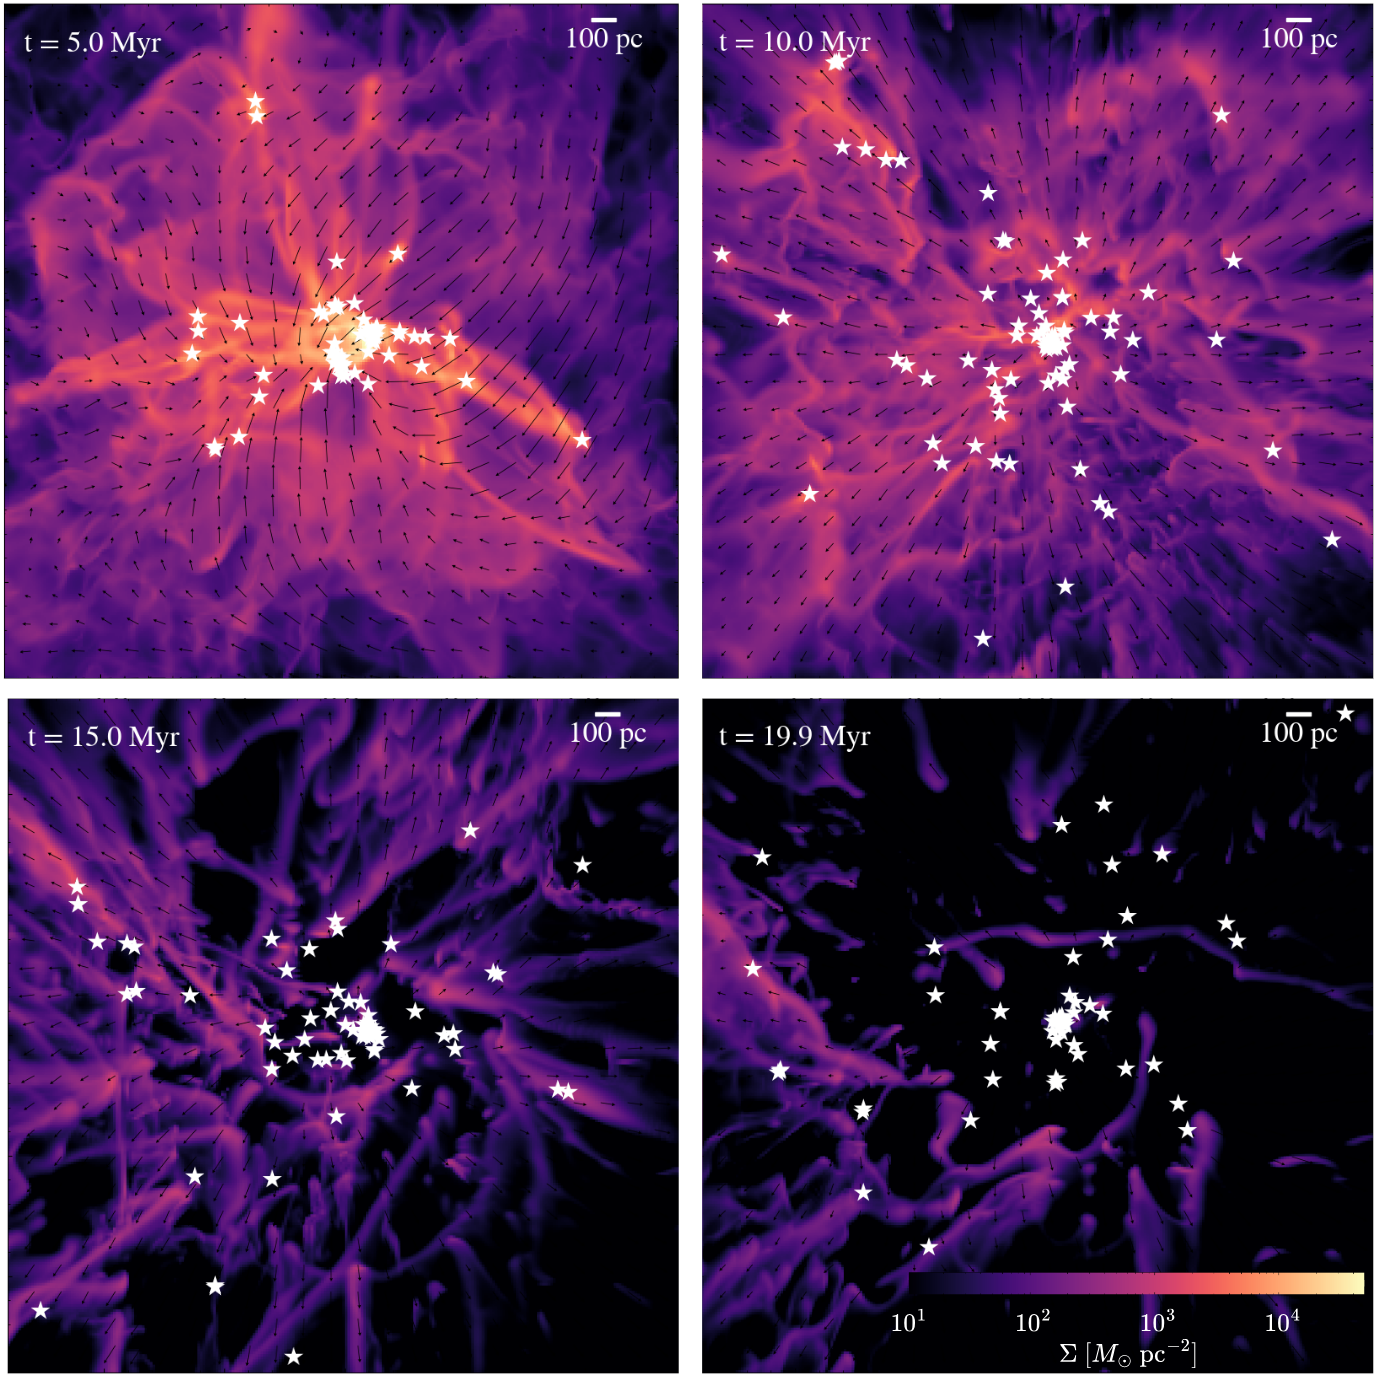
\includegraphics[width=\linewidth]{fig1.png}
    \caption{Frames from the fiducial simulation ($\mathtt{SNeRHD,f}$) at t = 5, 10, 15, 20 Myr. The colorbar indicates the surface density of gas, integrated along the z axis over the full length of the box, $2R = 1.4\ \mathrm{kpc}$.}
    
    \label{fig1:intro}
\end{figure*}


\begin{figure}[ht!]
    \centering
    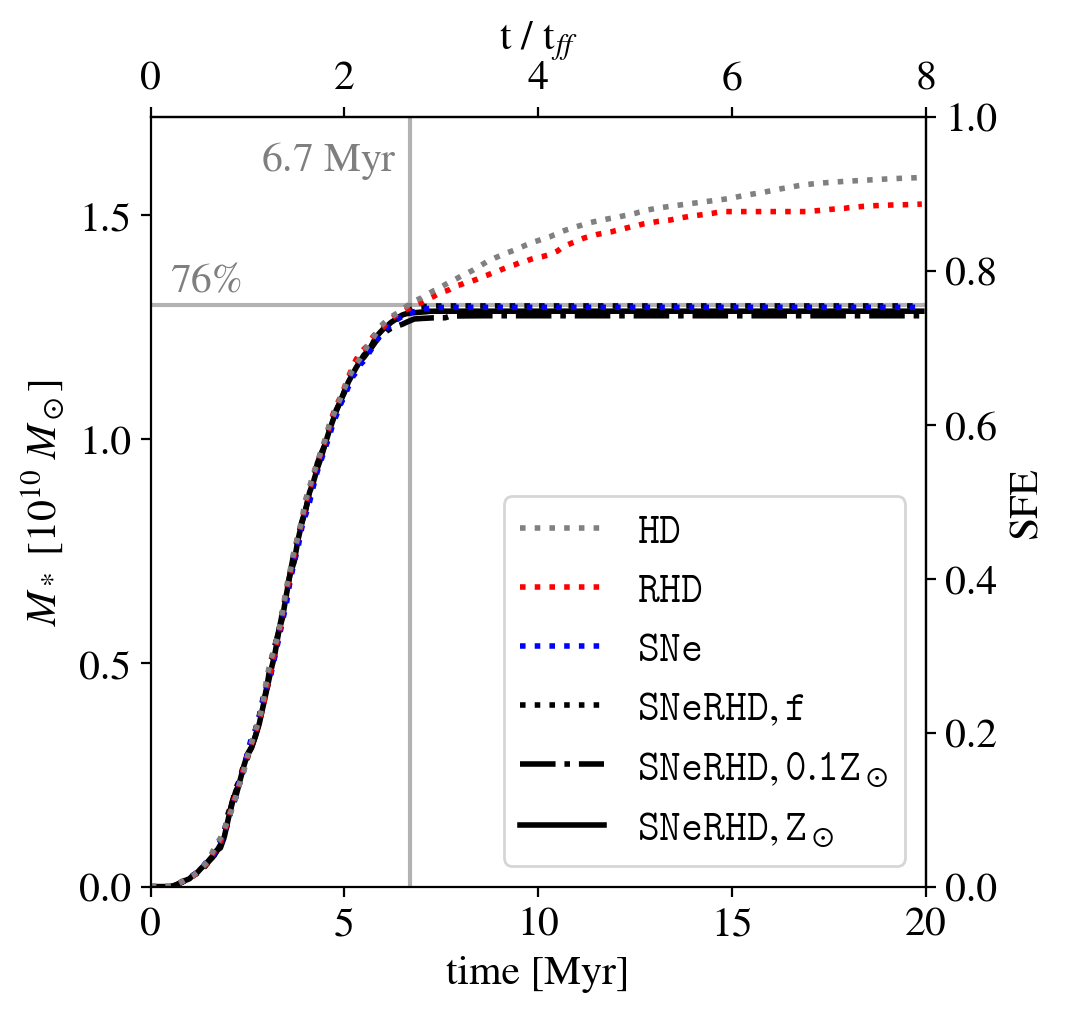
\includegraphics[width=\linewidth]{fig2.png}
    \caption{Star formation efficiency of the simulation runs presented in this work (Table 2). The color of each line indicates the feedback physics included, while the linestyle encodes the metallicity of the gas. The vertical dashed line indicates the detonation of the first supernova at t = 6.3 Myr. The horizontal dashed line shows the peak SFE achieved by the fiducial run $\mathtt{SNeRHD0.01Z_\odot }$.}
    \label{fig2:sfe}
    
\end{figure}

The dynamical evolution of the clouds is primarily governed by the competition between gravity and stellar feedback. At early times, gravitational contraction dominates, aided by supersonic shocks that compress the gas into dense filaments. The gas has a freefall time of $t_\mathrm{ff} \approx 2.5\ \mathrm{Myr}$, and the first star clusters form within the first 1 Myr of the simulations. 

Figure \ref{fig1:intro} shows snapshots of the fiducial run, $\mathtt{SNeRHD}$, at t = $(2,4,6,8) \times t_\mathrm{ff}$ , which correspond to 5, 10, 15, 20 Myr. At $5\ \mathrm{Myr}$, the gas is undergoing global radial infall. By this point, $10^9\ M_\odot$ of star clusters have already formed, which are primarily located in the center of the domain. Filaments funnel gas into the center of the domain, fueling continued star formation.

By 10 Myr, the dynamical balance has shifted and the large-scale velocity of the gas is radially outward. Between 10 Myr and 15 Myr, $\sim 1.5\times 10^9\ M_\odot$ of gas has been removed from the domain by feedback, leaving behind diffuse tendrils in place of dense filaments. An additional $4\times 10^8\ M_\odot$ of gas is lost between $15-20$ Myr, and the remaining gas is at the periphery and moving outward. By $t= 20$ Myr, there is $2\times 10^8\ M_\odot$ ($1\%$ of the $M_\mathrm{g,0}$) left in the simulation box along with an unobscured, tightly bound set of star clusters. In the following section, we discuss the relative contributions of radiation and supernova feedback in shaping the dispersal of the interstellar medium (ISM).

\subsection{Outflows driven by supernovae}
Figure \ref{fig2:sfe} shows the integrated star formation efficiency (SFE) as a function of time, 
\begin{align}\label{eq1:sfe}
    \epsilon_* \equiv \frac{M_*}{M_{g,0}}
\end{align}
where $M_*$ is the stellar mass, and $M_{g,0}$ is the initial mass of the gas cloud. All the simulation runs reach $\epsilon_* \sim 20\%$ within one freefall time ($t_\mathrm{ff}=2.5$ Myr), independent of feedback physics or metallicity. By $2t_\mathrm{ff}$, $\epsilon_* \sim 65\%$ for all the runs.% \textcolor{red}{and there still hasnt been enough time for jets ?}.

$M_*$ increase monotonically in the hydro-only run ($\mathtt{HD}$), ultimately reaching an SFE of $\gtrsim 93\%$. The $\mathtt{RHD}$ run follows a similar trend, reaching an SFE of $\epsilon_* = 90\% $ by the simulation end at $t = 8t_\mathrm{ff}$ Myr. 

For a given stellar population, the ratio between radiation pressure from UV photons and the force of gravity is given by:
\begin{align}\label{eq2:Guv}
    \Gamma_\mathrm{UV} = \frac{L_\mathrm{UV}/M_* }{4\pi c G\Sigma}
\end{align}
where the specific UV luminosity is $L_\mathrm{UV}/M_* = 900\ L_\odot M_\odot^{-1}$ for a Chabrier IMF, and $\Sigma$ is the surface density of gas in the ISM \citep{2024ApJ...967L..28M}. Gas with surface densities in excess of $\Sigma_\mathrm{crit} \gtrsim 10^3 M_\odot\ \mathrm{pc^{-2}}$ would have $\Gamma_\mathrm{UV}$ less than unity, favoring gravitational contraction. 

Collapse dominates throughout the runtime of the $\mathtt{RHD}$ simulation, leading to the formation of a bound, coherently rotating disk of gas around the star clusters that is morphologically indistinguishable from the gas in the $\mathtt{HD}$ run. The inability of radiation pressure to regulate star formation in clouds with $\Sigma_\mathrm{gas} > \Sigma_\mathrm{crit}$ is consistent with analytical solutions \citep{2010ApJ...710L.142F,2019MNRAS.483.5548G} and cloud-scale RHD simulations \citep{2023MNRAS.521.5160M}.

% \begin{align}
% \frac{F_\mathrm{UV}}{F_\mathrm{grav}} \sim \frac{\epsilon_* M\langle \sfrac{\dot{p}_*}{M_*}\rangle}{\sfrac{GM^2}{R^2}},
% \end{align}

% where $\langle \sfrac{\dot{p}_*}{M_*}\rangle$ is the rate of specific momentum injection by radiation \citep{2019MNRAS.483.5548G}. Neglecting gas self-gravity, the ratio of the gravitational pressure to the Eddington pressure from UV radiation is given by

By contrast, the $\mathtt{SNe}$ and $\mathtt{SNeRHD}$ runs stop forming stars after $t = 6.7$ Myr and plateau at $\epsilon_* \sim 75\%$ (Figure \ref{fig2:sfe}). This coincides with the detonation of the first supernovae, which shock the ISM to $T \sim 10^7\ \mathrm{K}$ and ionize it(Figure \ref{fig3:phase_diagram}). In addition to quenching star formation, the feedback from supernovae is responsible for disrupting the ISM and driving radial outflows (Figure \ref{fig4:postage_fbks}). Taken together, these results indicate that supernova feedback constitutes the dominant mechanism capable of halting star formation for dense gas clouds, such as those in the early universe. 

In the following section, we calculate the bulk dynamical properties of the outflows launched by supernovae.

\begin{figure*}[ht!]
    \centering
    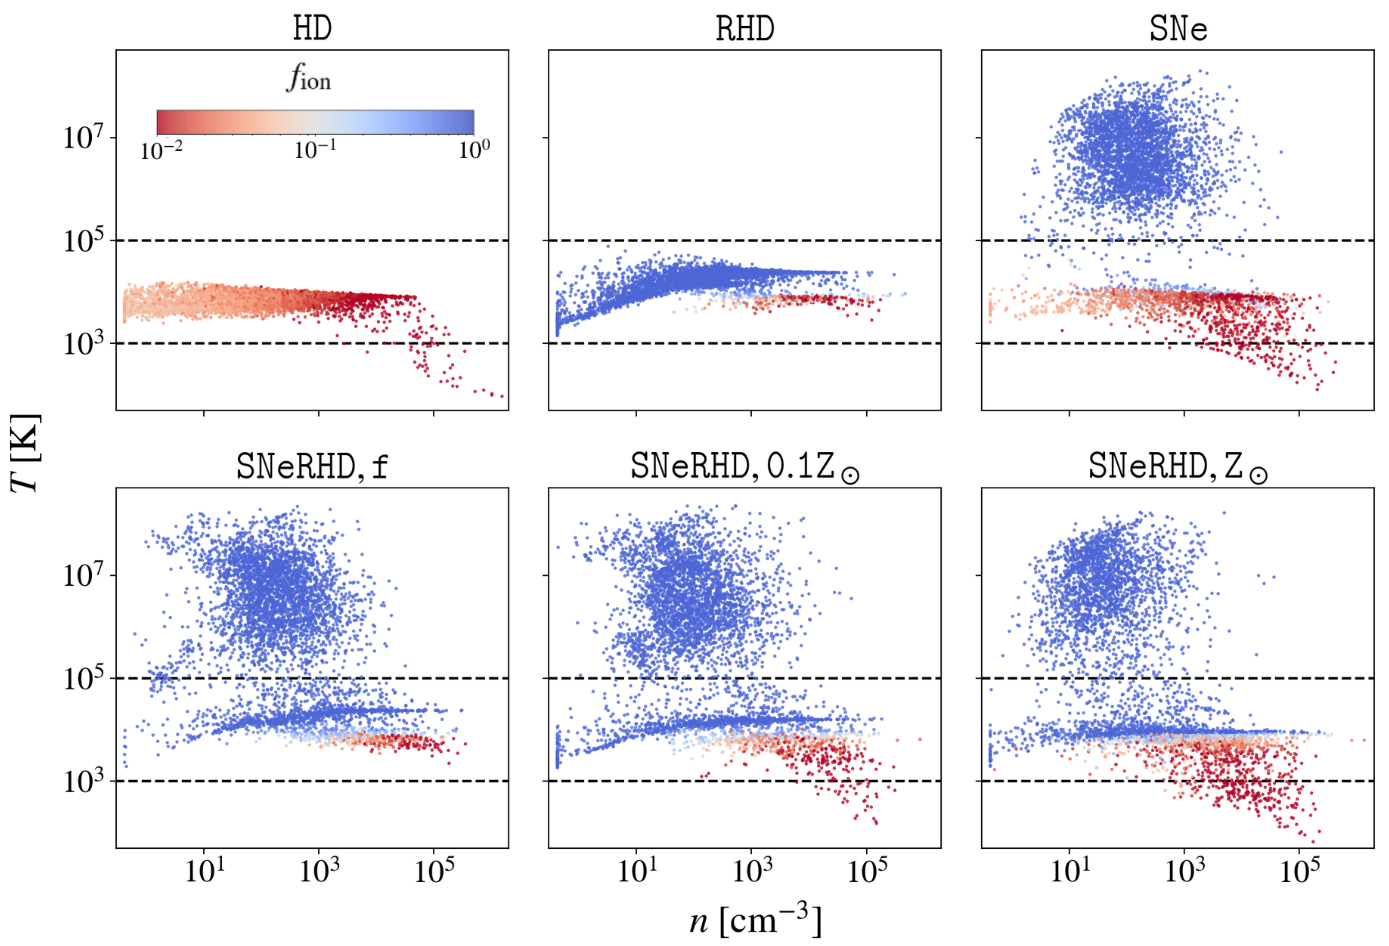
\includegraphics[width=\linewidth]{fig3.png}
    \caption{Phase-diagram of the interstellar gas at t = 10 Myr. The color of the scatter points indicates the ionization fraction, and the pair of horizontal lines show $T = 10^3$ and $T = 10^5$ K, which demarcates between the cold/warm and warm/hot phases respectively}
    \label{fig3:phase_diagram}
\end{figure*}

\begin{figure*}[ht!]
    \centering
    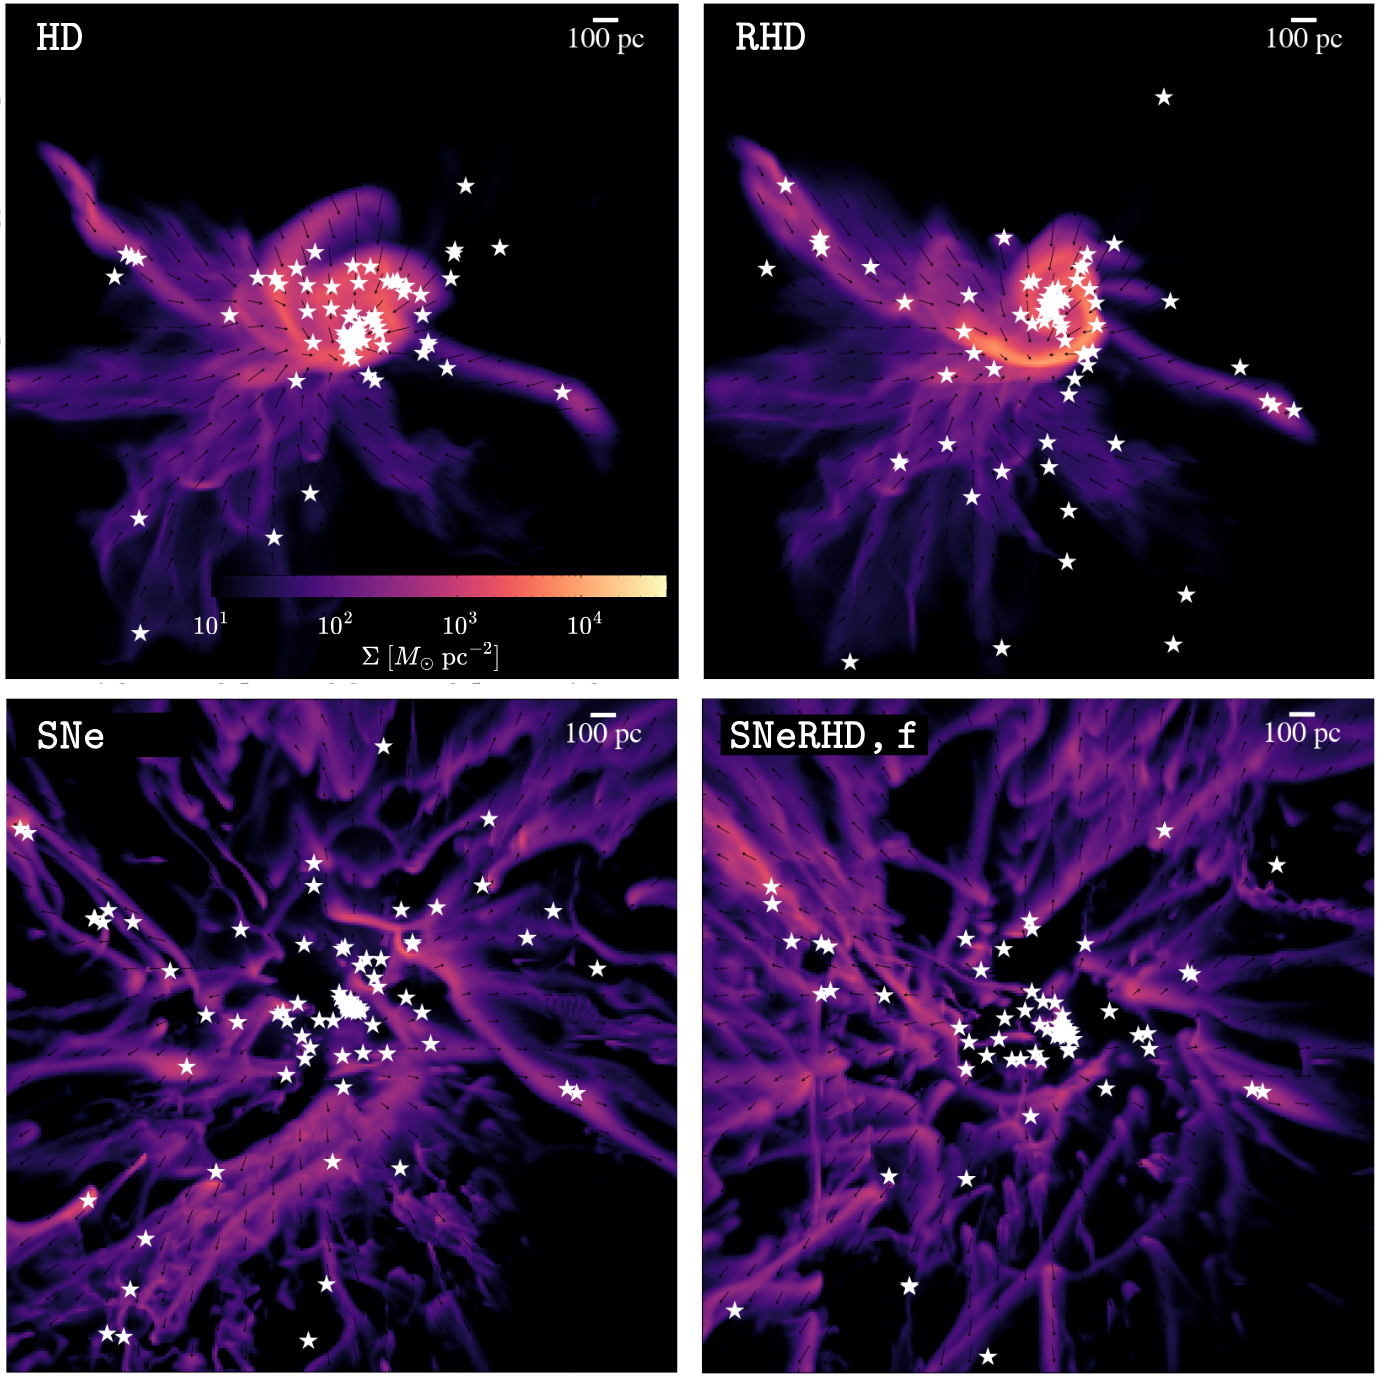
\includegraphics[width=\linewidth]{fig4.png}
    \caption{Snapshots at t = 15 My for the four different feedback cases. In the control ($\mathtt{HD}$) and radiation-only ($\mathtt{RHD}$) runs, the interstellar gas remains dense, gravitationally bound, and with primarily inward flow direction. On the other hand, the gas in the $\mathtt{SNe}$ and $\mathtt{SNeRHD}$ runs has been dispersed by supernovae and is moving radially outward.}
    \label{fig4:postage_fbks}
\end{figure*}

% \newpage
\subsection{Evolution of supernova-driven outflows}
\begin{figure*}[ht!]
    \centering
    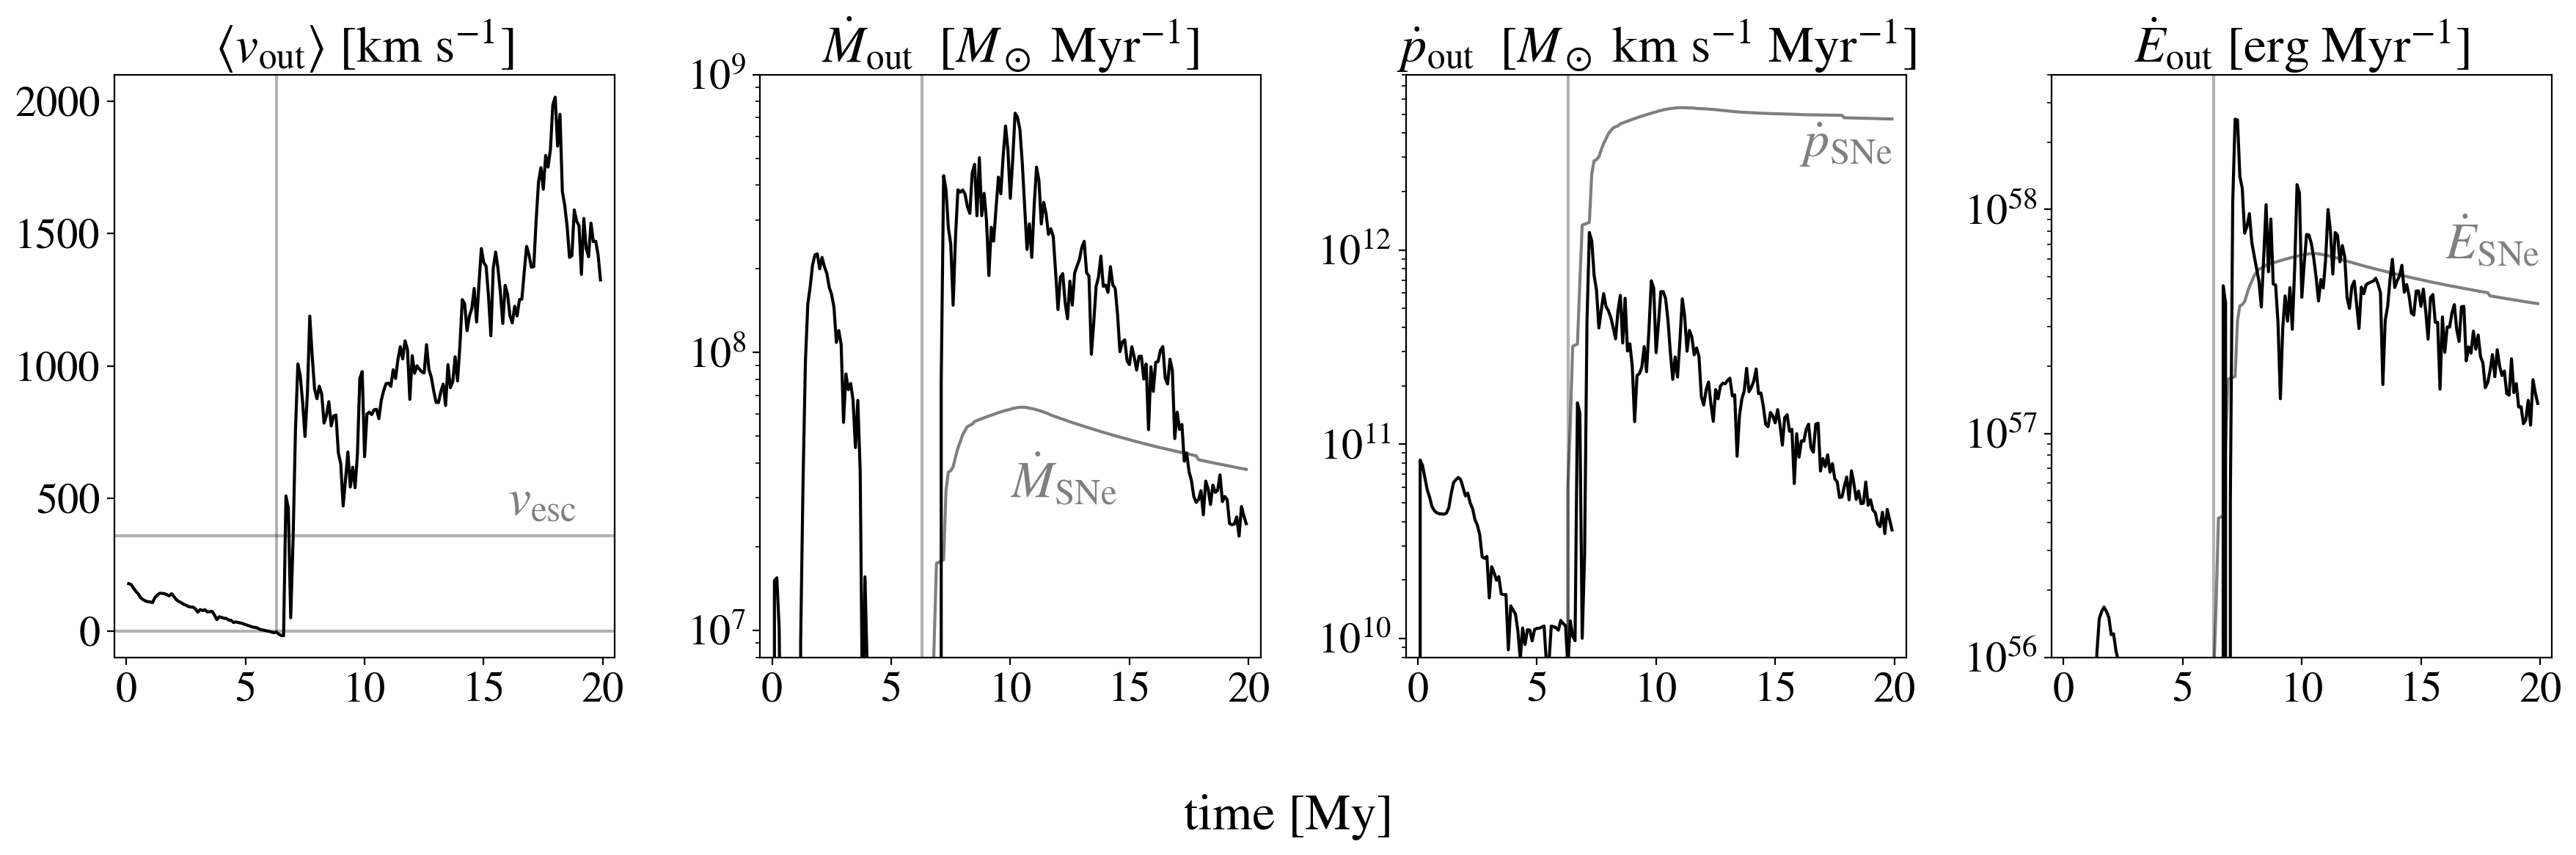
\includegraphics[width=\linewidth]{fig5.png}
    \caption{Outflow properties of the fiducial simulation: mass (left), average velocity (middle left), momentum (middle right), and energy (right). The vertical dashed line in each panel indicates 6.7 Myr, when the first supernova detonates. The dashed horizontal line in the second panel shows the velocity of the baryon potential is $360\ \mathrm{km\ s^{-1}}$. The grey lines indicate analytically derived values for the per-supernovae rate of mass, radial momentum, and energy injection.
    % \textcolor{red}{rearrange this+6,7 to be m,v,p,e, add a) b) c) d)}
    }
    \label{fig5:outflow_rates}
\end{figure*}

The rate of supernovae, $\dot{N}_\mathrm{SNe}$, in the simulations is insensitive to radiation and metallicity, rising steeply to a peak of $6\times10^4\ \mathrm{Myr}^{-1}$ at $10\ \mathrm{Myr}$ across all the runs. After this, the rate of detonation declines as the massive stars have died off, reaching to $\dot{N}_\mathrm{SNe} \sim 3\times10^4\ \mathrm{Myr}^{-1}$ at the simulation end time of $20\ \mathrm{Myr}$. Each supernova deposits an average kinetic energy of $10^{51}\ \mathrm{erg}$ into the ISM, along with $\sim 10 M_\odot$ of stellar material as ejecta. % \textcolor{red}{this propagates through the surrounding gas and pushes on it outward}

The mass flux of gas through a surface in the simulation box is given by: 
\begin{align}
    \dot{M}_\mathrm{out} = \int_{\partial S} \rho \ (v \cdot \hat{n})\ dA
\end{align}
where $\rho$ is the mass density of gas in each cell, $\hat{v}$ is its velocity, and $\hat{n}$ is the unit vector normal to the surface of the shell. The integral is evaluated over a Cartesian surface, following the methodology described in \cite{2023MNRAS.521.5160M}. 

Figure \ref{fig5:outflow_rates} shows the temporal evolution of $\dot{M}_\mathrm{out}$ through a surface at $r = 1\ \mathrm{kpc}$ in the fiducial run. An initial peak in $\dot{M}_\mathrm{out}$ occurs at $t \sim 2$ Myr from turbulent velocity fluctuations in the gas, which are subsequently damped as gravity begins to dominate and accretes gas back toward the center of the simulation. A second, more prominent spike of $\dot{M}_\mathrm{out}$ occurs at $t \sim 6$ Myr, shortly after the the first supernovae detonate.

Due to the continuous deposition of momentum by the supernovae, a steady outflow rate of $\langle \dot{M}_\mathrm{out} \rangle \sim 3\times 10^8 M_\odot \ \mathrm{Myr^{-1}}$ is maintained for about 5 Myr. After $t = 13$ Myr, $\dot{M}_\mathrm{out}$ begins to decline, as there is progressively less gas left in the domain interior to $r = 1\ \mathrm{kpc}$ (Figure \ref{fig1:intro}). 
% \textcolor{red}{compare to \citep{2026ApJ..1000..158C}}

The mass-averaged outflow velocity is given by:
\begin{align}
\langle v \rangle _\mathrm{out} = \frac{\int_{\partial S} \rho \ (v \cdot \hat{n})\ \mathcal{H}(v\cdot \hat{n})(v\cdot \hat{r})\ dA}{\int_{\partial S} \rho \ (v \cdot \hat{n})\ \mathcal{H}(v\cdot \hat{n})\ dA},
\end{align}
where $\mathcal{H}$ denotes the Heaviside step function applied to $v \cdot \hat{n}$ to filter for gas with a net outward velocity. 

During the gravitational collapse phase, the gas has velocities well below the $v_\mathrm{esc}$ of the system. The supernovae change this nearly instantaneously, accelerating the gas to $\langle v \rangle _\mathrm{out} \sim 1000\ \mathrm{km\ s^{-1}}$ at $t \sim 7$ Myr. As the amount of gas left in the simulation decreases with time, the supernovae impart a larger specific momentum to the gas. By t = 20 Myr, the outflows have $\langle v \rangle _\mathrm{out} \gtrsim 1500\ \mathrm{km\ s^{-1}}$, more than twice the escape velocity of the system.

Figure \ref{fig5:outflow_rates} also shows the momentum and energy fluxes carried by the outflows, which we calculate as:
\begin{align}
    \dot{p}_\mathrm{out} &= \int_{\partial S}\ \rho \ (v \cdot \hat{n}) (v \cdot \hat{r})\ dA \\
    \dot{E}_\mathrm{out} &= \int_{\partial S}\ \rho \ (v \cdot \hat{n})\ (\frac{v^2}{2} + \ \ e_\mathrm{int})\ dA.
\end{align}

The first (second) term in the integrand of $\dot{E}_\mathrm{out}$ correspond to the kinetic (thermal) energy of the gas. Both the momentum and energy flux exhibit behavior qualitatively similar to $\dot{M}_\mathrm{out}$, rising sharply following the onset of supernovae and subsequently declining as gas is expelled from the system. 

The rate at which the supernovae inject radial momentum into the surrounding ISM, $\dot{p}_\mathrm{SNe}$, depends on the ambient density and metallicity: $2.8\times 10^5 (\frac{n}{n_0})^{-1/7}\ (\frac{Z}{Z_0})^{-2/7}\ M_\odot\ \mathrm{km\ s^{-1}}$ \citep{2023ApJS..264...10K,1988ApJ...334..252C}. for gas with  $n_0 = $,and $Z_0 = Z_\odot$,  $\dot{p}_\mathrm{SNe} = 4\times 10^{12} M_\odot\ \mathrm{km\ s^{-1}\ Myr^{-1}}$, more than an order of magnitude larger than flux $\dot{p}_\mathrm{out}$ of the gas. While radial momentum is not conserved in the outflows, the total energy flux remains approximately constant at $\sim N_\mathrm{SNe} \times 10^\mathrm{51}$ erg, indicating that the outflows are energy-conserving. 

In this regime, the winds retain the full mechanical energy injected by the supernovae, giving them an increased ability to quench star formation and launch the metal-rich ejecta into the circumgalactic medium \citep{1985Natur.317...44C}. This also indicates that the outflowing gas is unable to cool efficiently to radiate thermal energy. The lack of radiative cooling means that different temperatures of gas in the ISM do not have thermal exchange, leading to an outflow with a multi-phase structure. In the section below, we investigate the thermal structure of the outflows.

\subsection{Phase structure of outflows}
\begin{figure*}[hb!]
    \centering
    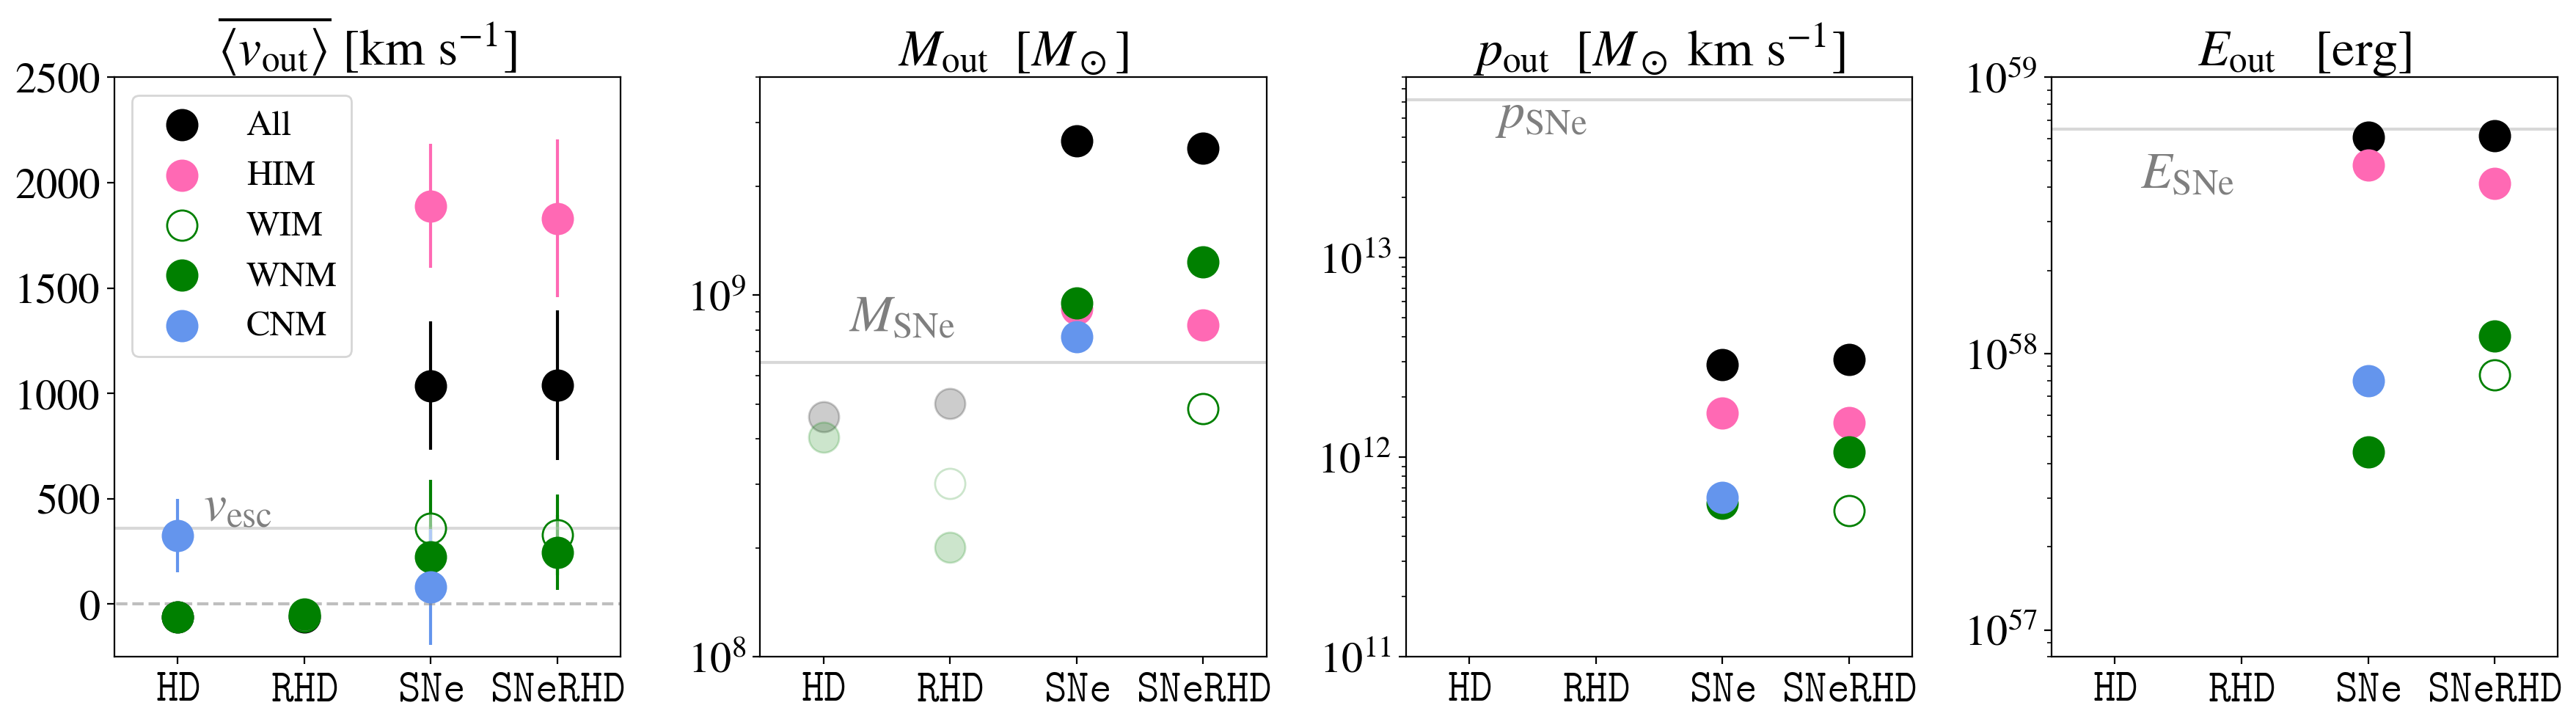
\includegraphics[width=\linewidth]{fig6.png}
    \caption{Left to right: the average outflow velocity, total mass, momentum and energy carried by the outflows through a surface at r = 1000 pc. The vertical lines on each data point in the velocity panel indicate the 1-$\sigma$ variation of the velocity over the period $t \in (6.7, 20) \ \mathrm{Myr}$. The $\mathtt{HD}$ and $\mathtt{RHD}$ runs have a net inflow, while the runs with supernova feedback have a net outflow. The marker colors indicate the phase of the gas, and the dashed horizontal lines in the second row show the maximum theoretical yields. 
    % \textcolor{red}{separate by thermal and kinetic energy -- circle vs square, and that will enable separating out what are the radiative energy losses vs kinetic}
}
    \label{fig6:terminal_mpe_phases}
\end{figure*}

The thermal and ionization state of the ISM is dependent on both the feedback physics and the metallicity of the simulations (Figure \ref{fig3:phase_diagram}). In this work, we define gas with temperatures of $T < 10^3\ \mathrm{K}$ to constitute the cold phase and gas with $T \geq 10^5\ \mathrm{K}$ as the hot phase. The hot gas is completely ionized (HIM), while the cold gas is completely neutral (CNM). The warm gas, which exists at intermediate temperatures of $T \in (10^3,\ 10^5)\ \mathrm{K}$), is split into the WNM ($f_\mathrm{ion} < 0.5$) and WIM ($f_\mathrm{ion} \geq  0.5$). 

At $t = 10$ Myr, the gas in the $\mathtt{HD}$ run consists of dense CNM ($n > 10^5\ \mathrm{cm^{-3}}$) and WNM at $ \lesssim 10^4$ K covering a wide range of densities $n \in (10^{-1}, 10^5)\ \mathrm{cm^{-3}}$. Due to the UV radiation emitted by the stars, the ISM in the $\mathtt{RHD}$ run is moderately warmer, and significantly ($> 40\%$ ionized. Supernova feedback introduces the HIM, which has $n \in (10^1, 10^3)\ \mathrm{cm^{-3}}$ and makes up $9\%$ of the gas in the simulation at this time. The remaining $91\%$ of the gas is in the warm phases, which is primarily ($55\%$) neutral. 
% On the other hand, there is no cold gas in the $\mathtt{SNeRHD}$ run, and the warm phase is primarily (\textcolor{red}{fraction} ionized).

The velocity of the gas in the $\mathtt{HD}$ and $\mathtt{RHD}$ is dominated by inflow over the whole course of the simulations (Figure \ref{fig6:terminal_mpe_phases}). On the other hand, both simulations with supernovae have HIM with average velocities of $1800\ \mathrm{km\ s^{-1}}$ over this same period. The WNM and WIM have outward velocities of $\sim 300$ ($0.5 v_\mathrm{esc})$ in $\mathtt{SNe}$ and $\mathtt{SNeRHD}$ runs.

The total gas mass transported by the outflows over the course of the simulation is: $$M_\mathrm{out} = \int_{t=6.7\ \mathrm{Myr}}^{20} \dot{M}_\mathrm{out} \Delta t.$$ $M_\mathrm{out}$ is approximately equal for the $\mathtt{SNe}$ and $\mathtt{SNeRHD}$ runs, $3\times 10^9\ M_\odot$. However, the partitioning of this total mass between the phases is different. There is no WIM without radiation, and the $\mathtt{SNe}$ outflows are made up of equal amounts of HIM and WNM ($\sim 10^9\ M_\odot$), with appreciable CNM ($8\times 10^8 M_\odot$). By contrast, in $\mathtt{SNeRHD}$, there is more mass in the WNM ($1.12\times 10^9$), negligible amounts of CNM, and the WIM ($5 \times 10^8 M_\odot$) in $\mathtt{SNeRHD,f}$ now makes up about $40\%$ of the total gas in the warm phase. There is about the same amount of HIM ($8.3\times 10^8 M_\odot$) as in $\mathtt{SNe}$, which is reflective of the similar rate of supernovae between the two runs.

While the HIM carries only about $30\%$ of $M_\odot$ in both runs $\mathtt{SNe}$ and $\mathtt{SNeRHD}$, it dominates the momentum and energy budget of the outflows due to its extreme velocities. 
% The hot winds in the $\mathtt{SNe}$ ($\mathtt{SNeRHD}$) run make up \textcolor{red}{$\gtrsim 60\%$ ($\gtrsim 60\%$)} of the total energy in the outflows. 
% \textcolor{red}{in the sne run, the energy is primarily kinetic? , while in the snerhd it is thermal?}.
This demonstrates that the supernova-driven winds are unable to radiate away thermal energy before they reach the surface at $\sim 1\ \mathrm{kpc}$.
% \textcolor{red}{why does the cnm overtake the wnm in p and e when it has smaller v and m?}
% \textcolor{red}{We also look at the fluxes through a surface at the edge of the simulation, r = 1.4kpc, and the energy is still dominated by thermal /  all the numbers are the same??}
The ability of gas to cool effectively is strongly sensitive to its metallicity, line cooling drives radiative losses at temperatures of $T\ \in (10^5,\ 10^7)\ \mathrm{K}$. In the following section, we discuss how the bulk outflow properties depend on gas metallicity.

\subsection{Outflow properties as a function of metallicity}
\begin{figure*}
    \centering
    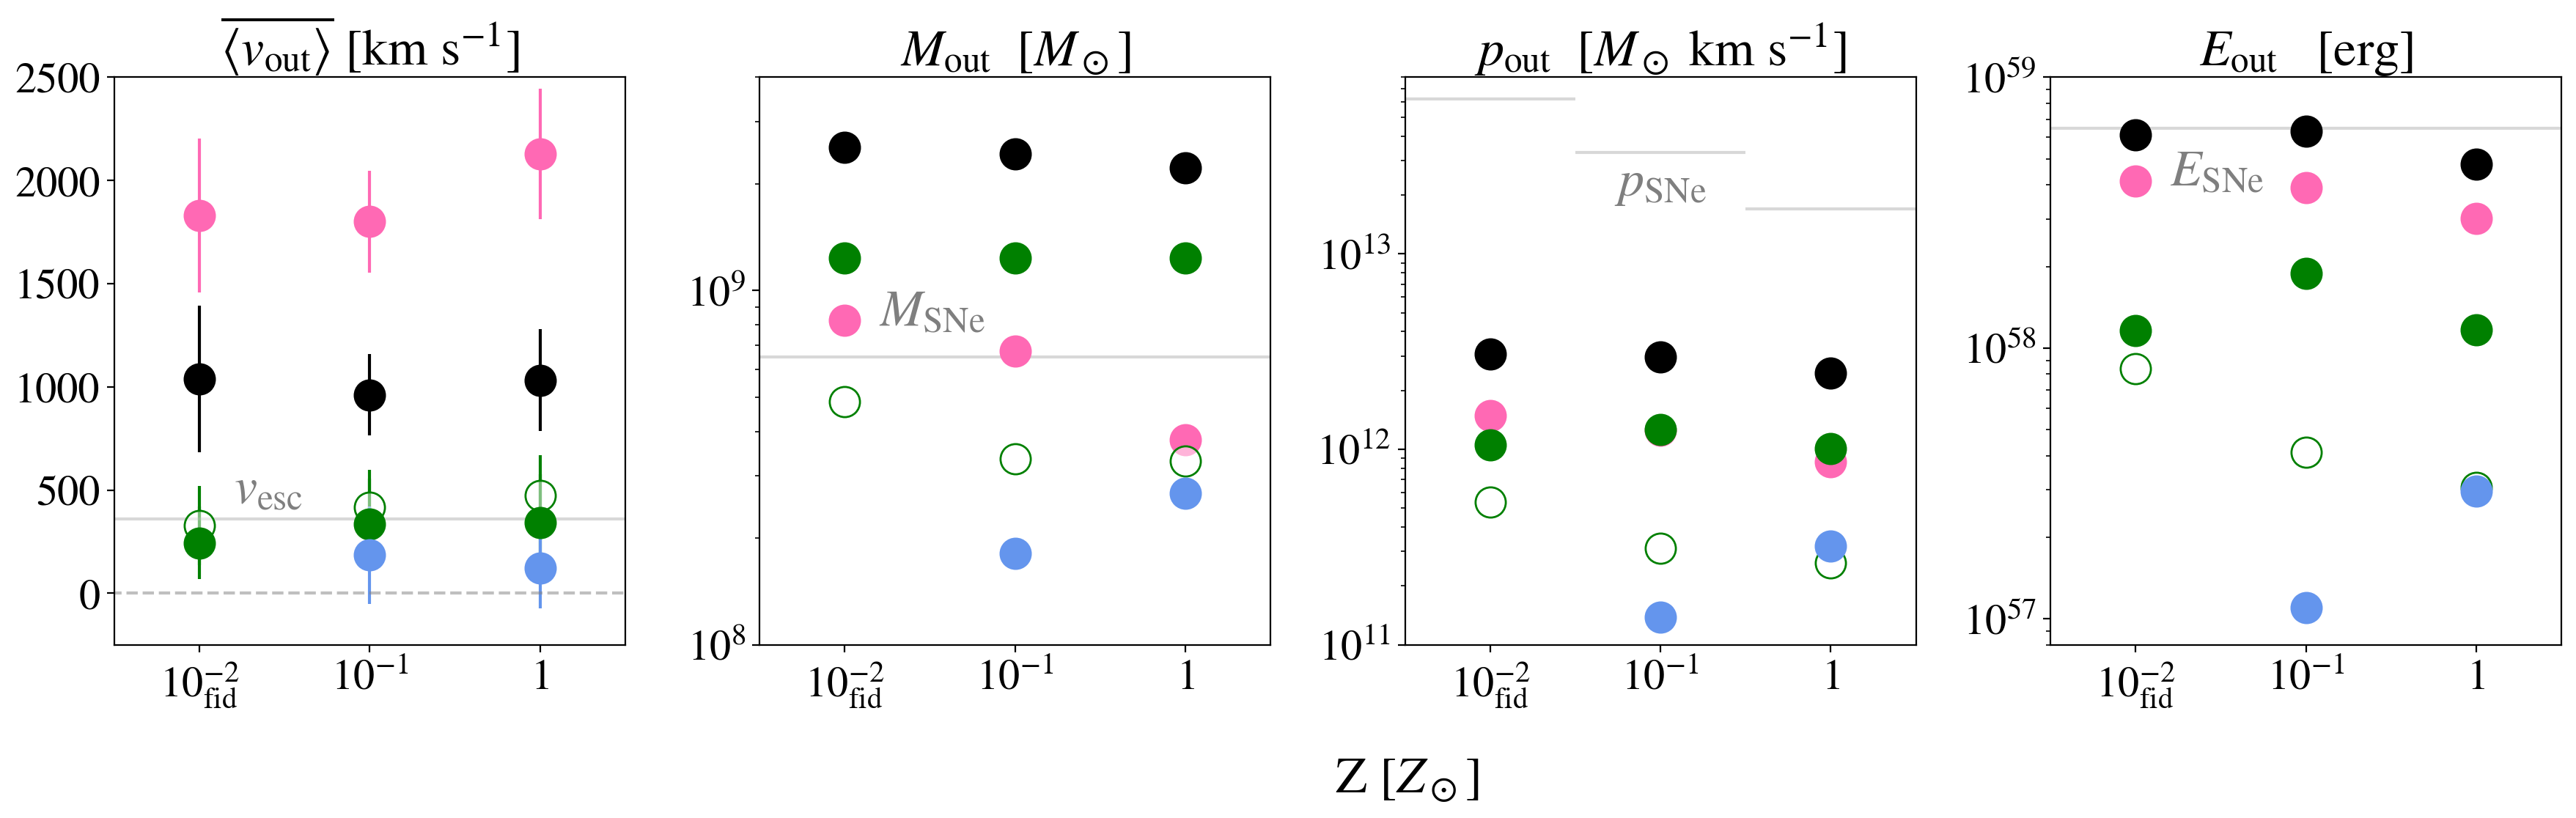
\includegraphics[width=\linewidth]{fig7.png}
    \caption{Same as Figure \ref{fig6:terminal_mpe_phases}, comparing the outflow properties with the gas metallicity.}
    \label{fig7:terminal_mtls_mpe}
\end{figure*}
The low metal and dust abundances at the fiducial metallicity ($0.01Z_\odot$) limit the radiative cooling efficiency of the hot gas in the $\mathtt{SNeRHD,f}$ run. Below, we examine how the thermal structure of the outflows change when the metallicity of the gas is increased by a factor of 10 and 100 in the $\mathtt{SNeRHD,0.1Z}_\odot$ and $\mathtt{SNeRHD,Z}_\odot$ runs, respectively. In Figure, \ref{fig7:terminal_mtls_mpe} we compare the bulk properties of the outflows--$\overline{\langle v_\mathrm{out} \rangle}$,$M_\mathrm{out}$, $p_\mathrm{out}$, $E_\mathrm{out}$-- in the $\mathtt{SNeRHD,0.1Z}$ $\mathtt{SNeRHD,0.1Z}$ $\mathtt{SNeRHD,0.1Z}$ runs. 

The total mass carried out remains broadly similar across the three metallicities, $2 \times 10^8 M_\odot$, as does the fraction of the $M_\mathrm{out}$ residing in the WNM. On the other hand, there is a systematic decrease in the HIM, with $M_\mathrm{out,HIM}$ being $20\%$ less in the $\mathtt{SNeRHD,0.1Z}_\odot$, and half in the  $\mathtt{SNeRHD,Z}_\odot$, in comparison to the fiducial run. The WNM also decreases, albeit moderately, (33\%) to $\approx 3\times10^8M_\odot$ in the higher metallicity runs. Correspondingly, the CNM now makes $8\%$ ($10\%$) of the wind mass at $Z=0.1Z_\odot$ ($Z=Z_\odot$). 

The outflow velocity averaged over the winds is broadly consistent across $\mathtt{SNeRHD,f}$,$\mathtt{SNeRHD,0.1Z}_\odot$, and $\mathtt{SNeRHD,Z}_\odot$, as is the relative speeds of the warm and hot phases. The velocity of the HIM increases moderately with metallicity, reaching $2100\ \mathrm{km\ s^{-1}}$ in the $\mathtt{SNeRHD,Z}_\odot$ run. Both warm phases also speed up with Z, with a $40\%$ increase in $\langle v \rangle$ from the fiducial metallicity to solar. The CNM, which was predominantly inflowing in $\mathtt{SNeRHD,f}$, is now part of the outflow. 
% \textcolor{red}{with velocities of $number \mathrm{km\ s^{-1}}$ at 0.1 zsun and zun.}

The partition of momentum and energy between the phases reflects the competing effects of the trends in mass and velocity. $p_\mathrm{out} \sim M_\odot \mathrm{km\ s^{-1}}$ across the three runs. $p_\mathrm{out,HIM}$ decreases by about $40\%$ from $0.01Z_\odot$ to solar metallicity, accompanied by an increase in the fraction of the total momentum residing in the WNM and CNM phases. 
% \textcolor{red}{much more radial momentum is conserved because the ejecta are cooling adiabatically?}

The total energy carried by the outflows also decreases with Z---while the $\mathtt{SNeRHD,0.1Z}_\odot$ and $\mathtt{SNeRHD,Z}_\odot$ runs are energy conserving ($E_\mathrm{out}\sim E_\mathrm{out}$), the energy of the winds at solar metallicit is $E_\mathrm{out}(Z_\odot) \sim 0.7 N_\mathrm{SNe} \times 10^{51}\ \mathrm{erg}$. This indicating that ISM gas in conditions more similar to the local universe radiatively cools more effectively. The greater phase separation between the HIM and the warm gas at higher metallicities suggests that the supernovae ejecta preferentially vent out of the cloud through low-density channels rather than sweeping up and uniformly accelerating the ambient ISM.

\subsection{Reionization}
\begin{figure*}[h!]
    \centering
    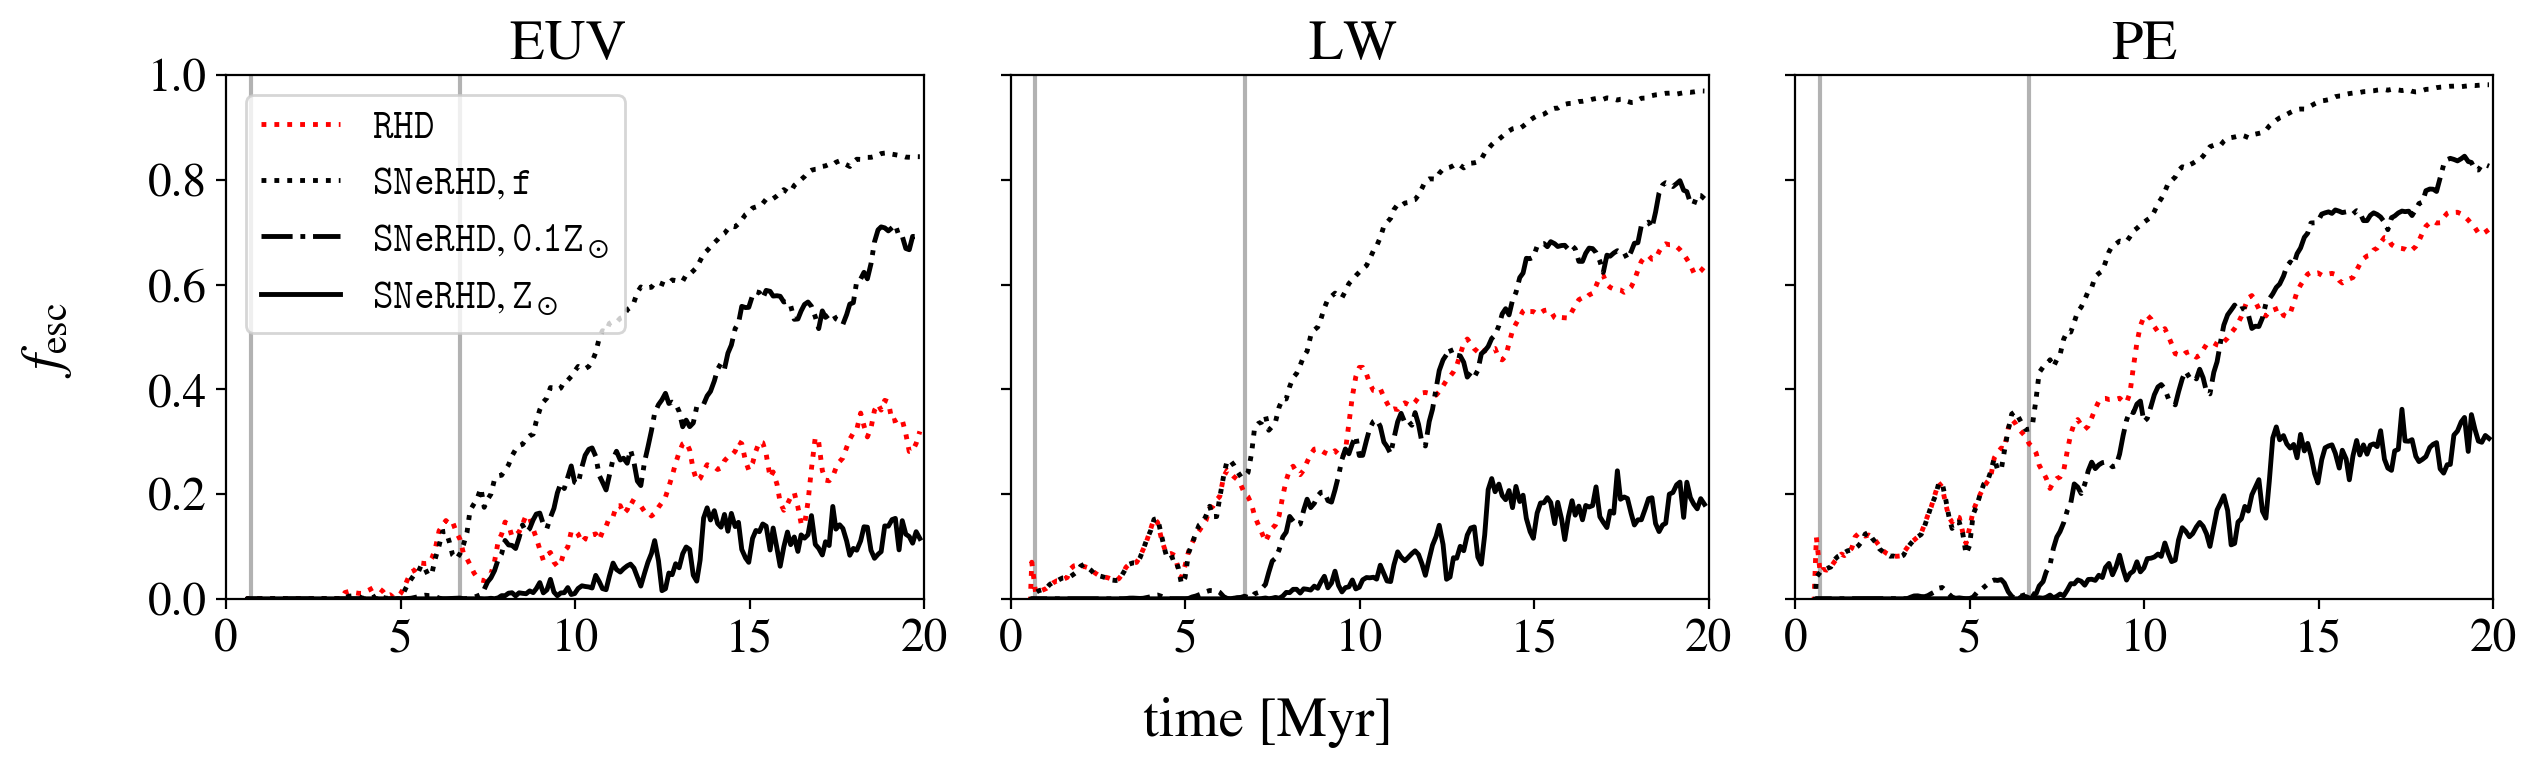
\includegraphics[width=\linewidth]{fig8.png}
    \caption{Escape fraction, $f_\mathrm{esc}$ of photons in the EUV (left), Lyman Werner (middle) and photoelectric (right) bands, for the runs with radiation feedback. The color of the lines indicates feedback physics, and the linestyle  encodes the metallicity. $f_\mathrm{esc}$ is systematically higher in the lower energy bands and shows a strong dependence on metallicity. }
    \label{fig8:fesc}
\end{figure*}
% The rest-frame UV luminosity of a starburst galaxy, as well as its capacity to ionize the surrounding intergalactic medium, depends on 
As the interstellar gas and dust are dispersed by supernova-feedback, the fraction of radiation that escapes the system, $f_\mathrm{esc}$, increases with time (Figure \ref{fig8:fesc}).  $f_\mathrm{esc}$ depends on the relative rates of absorption and emission of UV photons, given by: 
\begin{align}
    f_\mathrm{esc,\nu} = 1 - \left( \frac{\sum (\dot{E}_\mathrm{dust} + \dot{E}_\mathrm{gas})dV}{\sum_* L_{*}}\right)_\nu.
\end{align}
$L_{*,\nu}$ is the total luminosity of the stellar population in a given frequency band. The amount of radiation absorbed by gas and dust are $\dot{E}_\mathrm{x,\nu} = \kappa_x \rho c$, where the opacity of each species $\kappa_{x,\nu}$ is taken from \citep{2011ApJ...732..100D}.

We calculate $f_\mathrm{esc}$ in three frequency bands: extreme UV (EUV), Lyman-Werner (LW) and photoelectric (PE). EUV photons, with energies above $13.6\ \mathrm{eV}$, are absorbed by and ionize neutral hydrogen (HI). LW radiation, with energies $h\nu \in (11.2,13.6)\ \mathrm{eV}$, is absorbed by and dissociates molecular hydrogen, while the PE band, $h\nu \in (6,11.2)\ \mathrm{eV}$, is primarily absorbed by dust grains. 

In the $\mathtt{SNeRHD,f}$ run, LW and PE radiation begin escaping the system immediately upon the formation of the first star clusters, reaching $f_\mathrm{esc} = 20\%$ by $5\ \mathrm{Myr}$. This is shown in the sharp increase of $f_\mathrm{esc}$ in the $\mathtt{SNeRHD}$ run coincident with the onset of the first supernova explosions. After supernovae have been detonating for $\sim 5$ Myr, the escape fraction of LW (PE) photons has risen to $60\%$ ($80\%$). The $f_\mathrm{esc,EUV}$ rises more gradually compared to the other two bands, as the radiation must first ionize the surrounding HI before the system becomes transparent to EUV photons. 

The effect of supernovae on the escape fraction is most pronounced at the lowest metallicity, where approximately $80\%$ of EUV photons, and $\gtrsim 95\%$ of LW and PE escape the system by t = 20 Myr. At higher metallicities, the gas is more opaque to photons across all three bands, with $3$ (7) times less PE (EUV) radiation leaving the $Z=Z_\odot$ compared to the fiducial metallicity run. This is primarily because of the enhanced attenuation of PE photons by dust and the absorption of EUV and LW photons by the larger column densities of neutral gas.

As the UV photons propagates out of the starburst into the neutral IGM, an ionized bubble forms with a radius of:
\begin{align}
    R_\mathrm{ion} = (\frac{3Q_*}{4\pi n_z^2 \alpha_B})^{1/3},
\end{align}

where $Q_*$ is the amount of ionizing radiation emitted by the stellar population, and $\alpha_B = 4.2\times10^{13}\ \mathrm{cm^3\ s^{-1}}$ is the the HI ionization rate coefficient at T = $10^4$ K. We calculate the average number density of the IGM at $z = 10$ to be $$n_{10} = \frac{150H_0^2}{\pi Gm_p} = 2.2\times 10^{-3}\ \mathrm{cm^{-3}}$$ for a $\lambda-$CDM universe. The total amount of ionizing photons, $Q_*$ is calculated from the amount of radiation escaping the system:
\begin{align}
Q_* &= \frac{f_\mathrm{esc}L_\mathrm{EUV}}{\langle h\nu \rangle}, 
\end{align}
where $f_\mathrm{esc}$ and $L_\mathrm{EUV}$ are directly measured from the simulations, and we adopt the average photon energy $\langle h\nu \rangle = 18 \mathrm{eV}$ used for our LyC band.

We find that the sum of UV radiation escaping the starburst in $\mathtt{SNeRHD}$ produces an ionized bubble radius of approximately $2.8\ \mathrm{Mpc}$. Due to their lower $f_\mathrm{esc}$, the higher metallicity runs create smaller bubbles of $1.9\ \mathrm{Mpc}$ and $1.0\ \mathrm{Mpc}$ respectively. \textcolor{green}{what is the half-light radius of the system}
% \textcolor{red}{is this something observable / that people have looked at?}

% \citep{2020MNRAS.499.1395M} measure $R_{ion}$ and find
% \textcolor{red}{This ionized region would extend x of the distance to the nearest other galaxy of comparable size / luminosity. -> any other implications for reionization?} %given the (where does the uvlf = 1)  comoving number density of galaxies at z=10, this is () the average distance between them.

% 1/(alpha * n) is the recombination timescale, calculate and say in words



\section{Discussion}
\subsection{Outflow rainback time}

% \textcolor{orange}{how to factor in expansion / cooling into the how the velocity of the outflow changes with time? ratio of cooling time vs dynamical time - 1e4 ga yalut thats because its the equilibrium point bn cooling and heating - so if gas is there it will just stay there - large changes in the heating rate produce small changes in the equilibrium temperature bc the cooling rate of HI is baletinish index. the hot gas is so hot that its cooling time > dynamical time - adiabat hono evolve yaregal unless it shocks against the cgm - have as the end point to a radial 1d profile of kand T,rho wede lelaw yemihedbetn shape. drummond wind model does this - get out the cgms temperature structure 
% }

Below, we create a one-dimensional model for how the outflows evolve once they enter the CGM. We take $\langle v\rangle _\mathrm{out}$ averaged over t$ =6.7 - 20$ Myr as the launch velocity, and treat the outflow as a projectile moving through total gravitational potential of the system, $\Phi (r) = \Phi_\mathrm{bary}(r) + \Phi_\mathrm{DM}(r)$. This allows us to estimate the maximum distance that the gas travels to, $R_\mathrm{max}$, before being recycled back onto the system 

The baryonic potential $\Phi_\mathrm{bary}$ is calculated by treating the starburst as a spherically symmetric distribution of $M_* = \epsilon_* M_\mathrm{g,t0}$ with a radius of 500 pc (Figure \ref{fig1:intro}). The dark matter contribution, $\Phi_\mathrm{DM}$, is modelled as an NFW potential with a concentration parameter of $c=10$. 

The total gravitational potential of the system is then: 
\begin{align}
\Phi_\mathrm{tot}(r) = - \frac{G M_*}{r} - \frac{4\pi G \rho_0 R_s^3}{r}\ \ln\left(1 + \frac{r}{R_s}\right),
\end{align}
where $R_s = r_{200}/c = 1.3kpc$ is the scale radius of the dark matter halo, and $\rho_0 = \rho_c(z)2/3 \times 10^5 /(\ln 11 - 10/11)$ is its central density.

A gas parcel launched into $\Phi (r)$ with an initial velocity of $v_\mathrm{init} = \langle v_\mathrm{out} \rangle$ will have a total kinetic energy of:
\begin{align}
e_\mathrm{init} = \Phi(R_\mathrm{launch}) + \frac{1}{2}v_\mathrm{init}^2.
\end{align}

The phases of the outflow have dramatically different $v_\mathrm{init}$ across all the simulations. In the fiducial run, the HIM is launched with velocity of $1800\ \mathrm{km\ s^{-1}}$ from $R = 1\ \mathrm{kpc}$. Since $\langle v_\mathrm{out} \rangle_\mathrm{HIM}$ is much larger than $v_\mathrm{esc}$, the hot winds permanently escape the system, enriching the IGM.
% with the $M_\mathrm{out,HIM} \times f_d$, where \textcolor{red}{$f_d = number$ is the amount of dust and metals formed in the supernovae. cite someone from foley and co}. 

\begin{figure}[ht!]
    \centering
    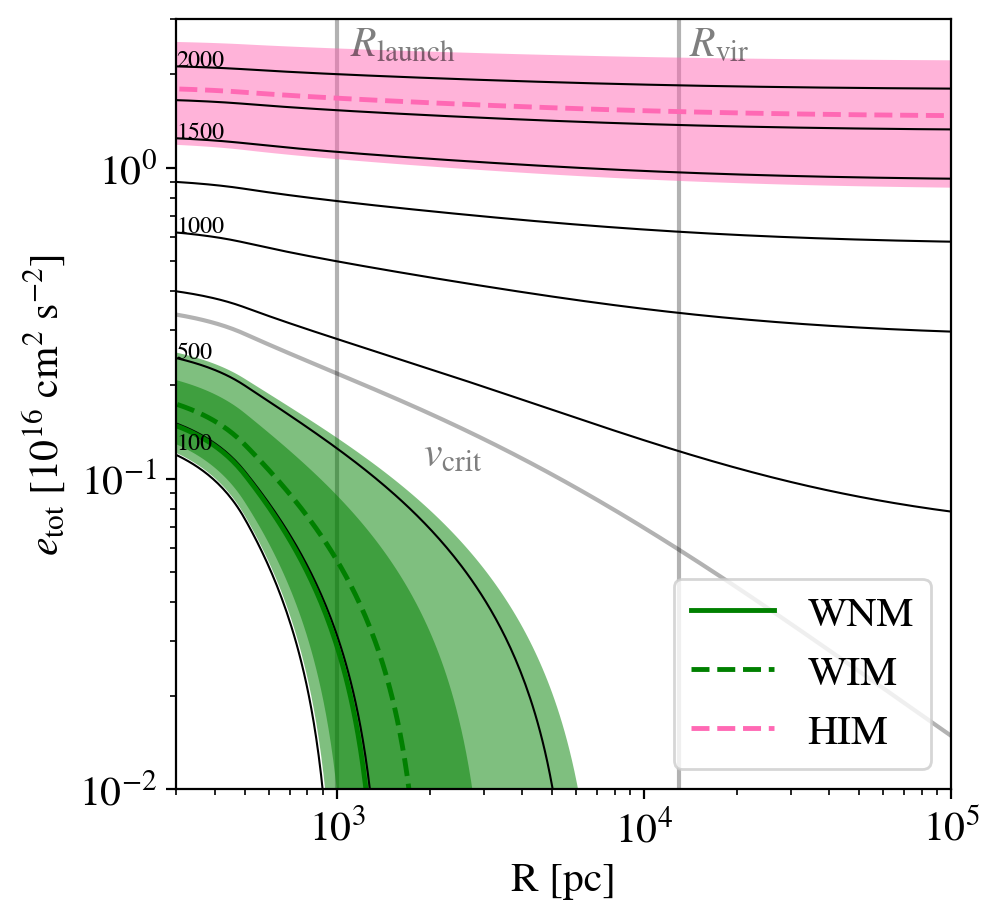
\includegraphics[width=\linewidth]{fig10.png}
    \caption{Kinetic of outflows in the fiducial simulation, where each color corresponds to a separate phase of the gas. The dashed and solid colored lines are the median velocity averaged over the period $6.7-20$ Myr. The shaded region correspond to the standard deviation of velocities over that same period.}
    \label{fig10:etot}
\end{figure}

The WNM and WIM, on the other hand, remain bound, since their launch velocities, $240\ \mathrm{km\ s^{-1}}$ and $330\ \mathrm{km\ s^{-1}}$, are well below $v_\mathrm{esc}$. To calculate the maximum radius $R_\mathrm{max}$ that warm gas reaches before being raining back onto the galaxy, we remember that winds are energy-conserving and set $e_\mathrm{init}(r) = e_\mathrm{tot}(R_\mathrm{max})$ for all $r$. By the definition of the maximum radius,
\begin{align}
    e_\mathrm{init} - \Phi(R_\mathrm{max}) = 0
\end{align}

Solving the above equation for each phase, we find that the WNM reaches a maximum radius of $\sim 1.4\ \mathrm{kpc}$ before raining back.The WIM is launched at a slightly faster velocity, so it gets to $\sim 2\ \mathrm{kpc}$.

The time it would take for the outflowing gas to return to the launch radius is $t_\mathrm{rain} = 2t_\mathrm{max}$, where $t_\mathrm{max}$ is given by:
\begin{align}
t_\mathrm{max} = \int_{R_\mathrm{launch}}^{R_\mathrm{max}}\sqrt{2(e_\mathrm{tot} - \Phi(r)\bigr)},
\end{align}

The WNM rains back onto the system after $6.1\ \mathrm{Myr}$, while the WIM travels for a total of $11.4\ \mathrm{Myr}$. These numbers are likely upper limits, since we don not here account for drag that the outflows would experience from the gas in the CGM. \textcolor{green}{how does this compare to the dynamical time of the system and is this something that could evolve into a UDG? -- when the gas rains back does it go all the way back to the r launch ketederegebet, or does it resettle at larger R}
% \textcolor{red}{how does this compare to: recent ferrara , somerville? paper on blue monster to red napping galaxy pipeline, and also what are the expectations for outflows based on the local universe}
% Thus, the starburst that is UV-bright at $z=10$ will be reobscured by an envelope of gas and dust weighing \textcolor{red}{total mass} by a redshift of \textcolor{cyan}{$z = x$}. 

% This suggests a plausible formation scenario for the heavily dust-obscured, red galaxies observed at $z=7$ by \textcolor{red}{e.g., ALMA / REBElS, in agreement with theoretical models ferrara paper about this}.
% Once the outflow material returns to the system, \textcolor{red}{implications for the lyminosity and color of the system}. 
\subsection{Comparison with simulations}
\textcolor{red}{Hydrodynamic simulations of conditions emulating both the local and early universe demonstrate that supernovae can drive energetic outflows that efficientyl remove gas and dust from galaxies (e.g.,\citealt{2026ApJ..1000..158C,2018MNRAS.481.3325F}). 

Cosmological zoom-in simulations provide a numerical counterpart to the set up described here \citep{
2025MNRAS.536..988F,2026arXiv260524104S,2026MNRAS.545f2119S,2025MNRAS.540.3350A}. \cite{2025MNRAS.540.3350A} run a cosmological zoom-in simulation of a halo with the same mass as presented in this work, $10^{11}\ M_\odot$. The galaxy undergoes several episodes of star formation between $z \in (14,\ 9)$, assembling a stellar mass of $3 \times 10^9 M_\odot$ by z = 9. The galaxy has an instantaneous SFR of $30-50\ M_\odot \ \mathrm{yr^{-1}}$, and an integrated SFE of $\epsilon \sim 0.1-0.3$.

The higher SFE in our simulations in comparison to \cite{2025MNRAS.540.3350A} reflects the physical differences of our set-ups. The simulations presented here each represent an isolated cloud, which lacks cosmological accretion history from the intergalactic medium. This new gas would decrease the star formation efficiency by keeping the total gas mass elevated. Additionally, the star formation in this work occurs in a single burst, while in \cite{2025MNRAS.540.3350A}'s case, accretion from the IGM both i) decreases the instantaneous SFE and ii) sustains star formation long-term by supplying fuel. 

\subsection{Comparison with analytical models}
% \textcolor{cyan}{background on the jwst observations and the theoretical models in response -- how to expand this beyond intro? and what portion of the time to tie back vs to talk about "the results we've gotten (mass loading factor etc(and also from before whose results have implications on the physics)}
\cite{2023MNRAS.522.3986F} proposed that once high-redshift galaxies cross a sSFR threshold of $25\ \mathrm{Gyr}^{-1}$, super-Eddington winds expel the interstellar dust and gas. In our simulations, we test whether the removal of the ISM by outflows is sufficient to render the young stellar population directly visible in the UV. 

The visual band extinction $A_\mathrm{V}$ in the $\mathtt{RHD}$, $\mathtt{SNeRHD,f}$, $ \mathtt{SNeRHD,0.1Z}_\odot$, and $\mathtt{SNeRHD,Z}_\odot$ runs is shown as a function of time in Figure \ref{fig9:muvav}. During the first 5 Myr, the fiducial metallicity runs have $A_\mathrm{v}\sim 3\ \mathrm{mag}$. During this same period, the $\mathtt{SNeRHD,0.1Z}_\odot$ ($\mathtt{SNeRHD,Z}_\odot$) run have 10x (100x) higher extinction, owing to the increased dust abundance in the ISM.

Once supernovae detonate and begin clearing the gas, $A_\mathrm{V}$ drops across all the metallicities, and produces an essentially dust-free stellar population with ($A_\mathrm{v} \lesssim 10^{-1}\ \mathrm{mag}$, in the the $\mathtt{SNeRHD,f}$ and $ \mathtt{SNeRHD,0.1Z}_\odot$ runs.
% This would produce an unattenuated starburst with blue UV slope $\beta_\mathrm{UV} \lesssim -2$, a scenario supported by analytical models of feedback-driven outflows (e.g., \citealt{2024A&A...684A.207F,2023MNRAS.520.2445Z}).
The clearing of the ISM by supernovae produces correspondingly larger jumps in the UV luminosity, which we discuss in the section below.

\subsection{Comparison with observations}

\begin{figure}%[ht!]
    \centering
    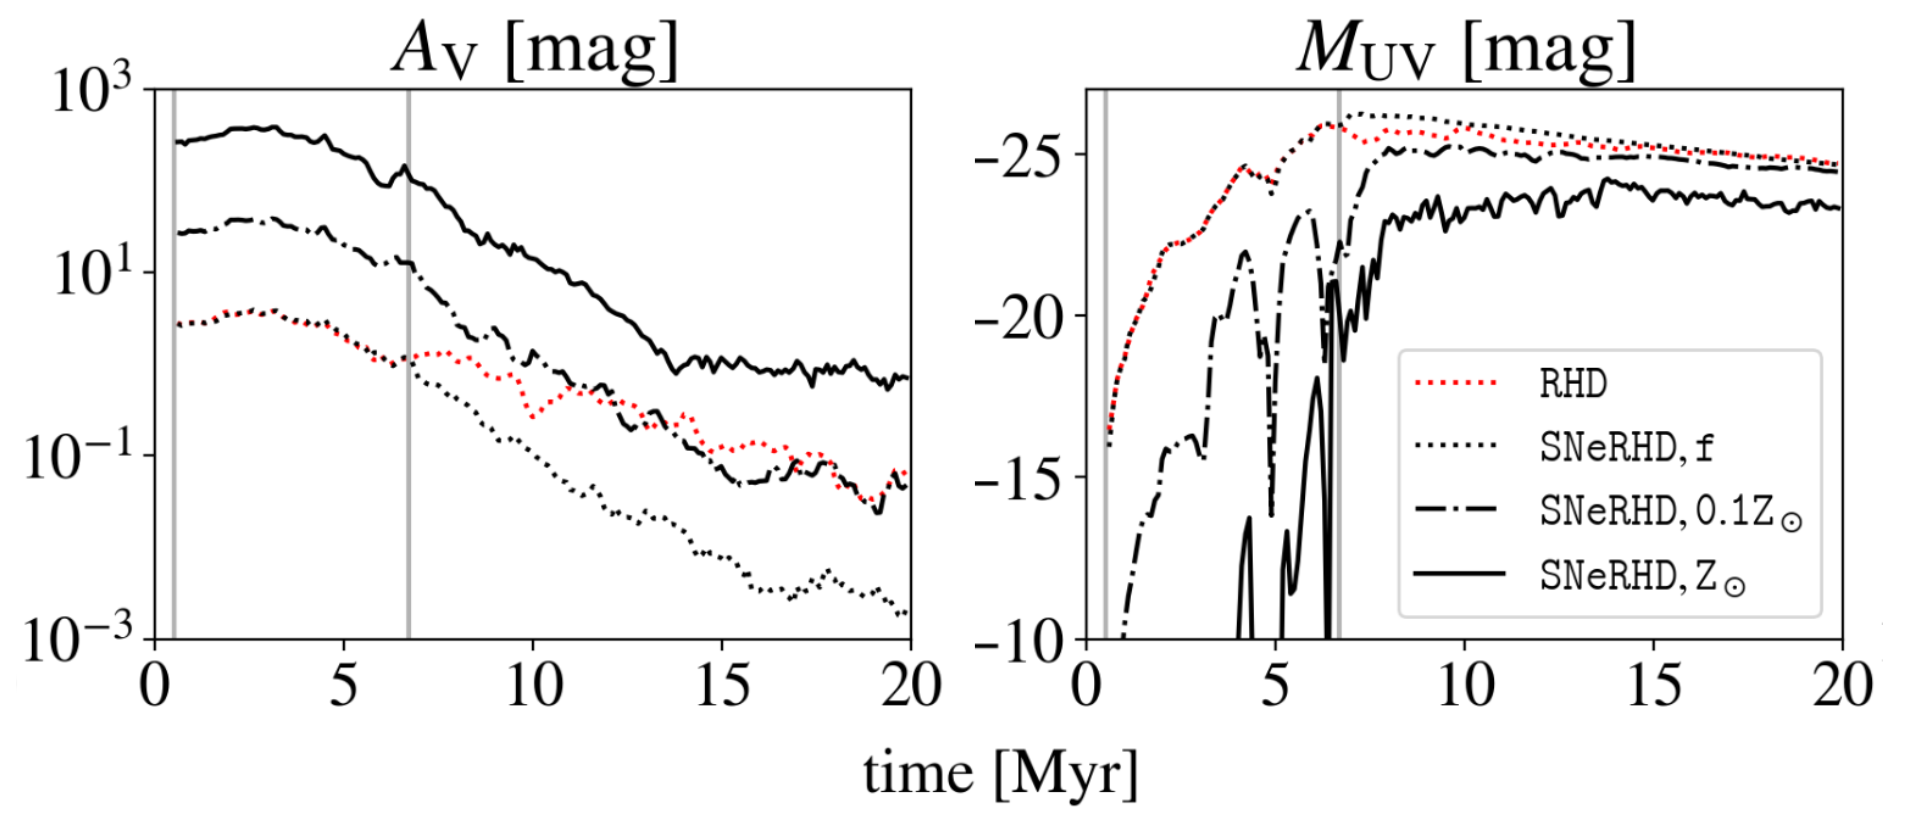
\includegraphics[width=\linewidth]{fig9.png}
    \caption{Rest-frame absolute UV magnitude, $M_\mathrm{UV}$ (left) and visual-band extinction of the system, $A_\mathrm{V}$ ( right) for the same simulations shown in Figure 8. The black lines are runs with both supernova and radiation feedback, while the red line is just RHD. The linestyles show the different metallicities of the gas}
    \label{fig9:muvav}
\end{figure}

The lowest-metallicity runs are have brighter $M_\mathrm{UV}$ across all times, reaching peak magnitudes near $M_\mathrm{UV} =-26$ mag shortly after 5 Myr (Figure \ref{fig9:muvav}). The difference between the $\mathtt{RHD}$ and $\mathtt{SNeRHD}$ remains $< 0.5 \mathrm{mag}$ even after the detonation of the first supernovae, indicating that the photoionization is sufficient to allow the escape of UV photons. Both runs become fainter at late times, consistent with the decreased UV output as the stars age and die, {$M_\mathrm{UV} \sim -25 \mathrm{mag}$. 

The massive galaxies observed by JWST at Cosmic Dawn have typical rest-frame UV magnitudes of $\sim -20\ \mathrm{mag}$ (e.g, \citealt{2024A&A...691A..87M})
While the extreme UV brightness of the simulated systems is in part a consequence of the large halo mass adopted in this work, when scaling $M_\mathrm{UV}$ down by $M_\mathrm{halo}$, we land on the observationally derived relation  \citep{2025MNRAS.543.3802Y,2025ApJ...985...80R}.

Metallicity has substantial effects on $M_\mathrm{UV}$, especially in the first 5 Myr. The dust-to-gas ratio of the $\mathtt{SNeRHD0.1Z}_\odot$ and $\mathtt{SNeRHD0.1Z}_\odot$ and $\mathtt{SNeRHDZ}_\odot$ runs is a factor of 10 and 100 larger than the fiducial case. This leads to increased absorption of UV photons by dust at higher Z, and the the $M_\mathrm{UV}$ remains faint during the gravitational collapse phase. The $Z = 10^{-1}\ Z_\odot$ run is on average $\sim 3\ \mathrm{mag}$ dimmer than the fiducial case, while $Z = Z_\odot$ run is $\gtrsim 10$ mag dimmer. Once the supernovae clear the gas, the higher metallicity brighten significantly, reaching $M_\mathrm{UV} \sim -23 $ by $t=20$ Myr. \citep{2026A&A...705L..10M}

\subsection{Caveats and Limitations}
\subsubsection{Resolution}
To check for numerical convergence, we run simulations at two different spatial resolutions, $128^3$ and $256^3$, for the four different feedback cases. Figure \ref{fig11:Ms_res} shows that independent of feedback physics,  the stellar mass formed per timestep is consistent with one another for the 20 Myr duration. Although the total stellar mass is the same, we find that the number of star clusters increases, with a proportional decrease in the the mass per cluster. Since the total stellar mass determines the momentum and energy deposited by supernovae, the bulk properties of the outflows remain the same across resolution. We therefore conclude that our primarily results are numerically converged.

After they have formed, the sink particles in our simulations are allowed to continuously accrete mass, which artificially decreases their age. This delays the onset of first supernova by approximately 2.5 Myr, about a freefall time. If the sink particle ages were not reduced in this way, e.g., by allowing multiple age bins per sink, the stellar population would age and die up to $t = 2.5$ Myr earlier, quenching star formation at $\epsilon_* \sim 0.5$.
% This much stellar mass would still produce enough supernovae to disperse the gas is still comparatively high}

    
\subsubsection{Interactions with the IGM}
The star formation efficiency (Equation \ref{eq1:sfe}) is dependent on the star formation rate and inversely dependent on the total gas mass. An actively star-forming system could still have low SFE if gas is being replenishing by accretion. The accretion rate for a $10^{11} M_\odot$ halo at $z = 10$, is $50$ Myr \citep{2025MNRAS.540.3350A}}, which is much longer than the whole run times, so the instantaneous star formation efficiencies reached are still realistic. They should be taken as an upper limit.
% ,since when integrating over time, in combination with the gas in the outflows raining back, the balance of star vs gas in these systems will eventually return to gas.

%bring back discussion about how the gas is going into the cgm without any push back or in  - so the rmax we calculate is an upper limit


\subsubsection{Neglect of Lyman-$\alpha$ scattering}
The radiation pressure on dust grains from reprocessed UV photons is the main mechanism of radiation feedback considered in this work. At metallicities of $\sim 10^{-2}\ Z_\odot$, Lyman-$\alpha$ radiation may impart significant momentum to the gas. At high HI columns, Ly-$\alpha$ photons near line center are subject to cross-sections $5.9\times 10^{-14}\ \mathrm{cm^2\ T_4^{-1/2}}$ \citep{2024ARA&A..62..529T}, causing them to undergo multiple scatterings before escaping \citep{2008MNRAS.391..457D,2008ApJ...681..771M}. Despite its physical importance, Ly$\alpha$ radiative transfer is computationally expensive to model accurately, due to its sensitivity to geometry, gas kinematics, and the need for ray-tracing \citep{2020MNRAS.497.3925L, 2022ApJ...934...37M}. 

Analytical approximations have shown that the momentum imparted by Ly-$\alpha$ resonance can exceed the radiation pressure of UV photons reprocessed by dust by factors of $\approx 300$ \citep{2021MNRAS.504...89T}, and exceed that of supernova-driven winds \citep{2018MNRAS.475.4617K}. This could potentially make Ly-$\alpha$ resonant scattering on par with supernovae on suppressing star formation (e.g., and driving neutral gas outflows (e.g., \citealt{2024ARA&A..62..529T, 2018MNRAS.475L.130A}). This makes the momentum imparted by supernovae a lower limit to the total possible that feedback can exert on the ISM. 
{\bf mike: update to mention Shyam's new paper with aaron smith, also olof nebrin's new 2D simulations paper}

\begin{figure}[ht!]
    \centering
    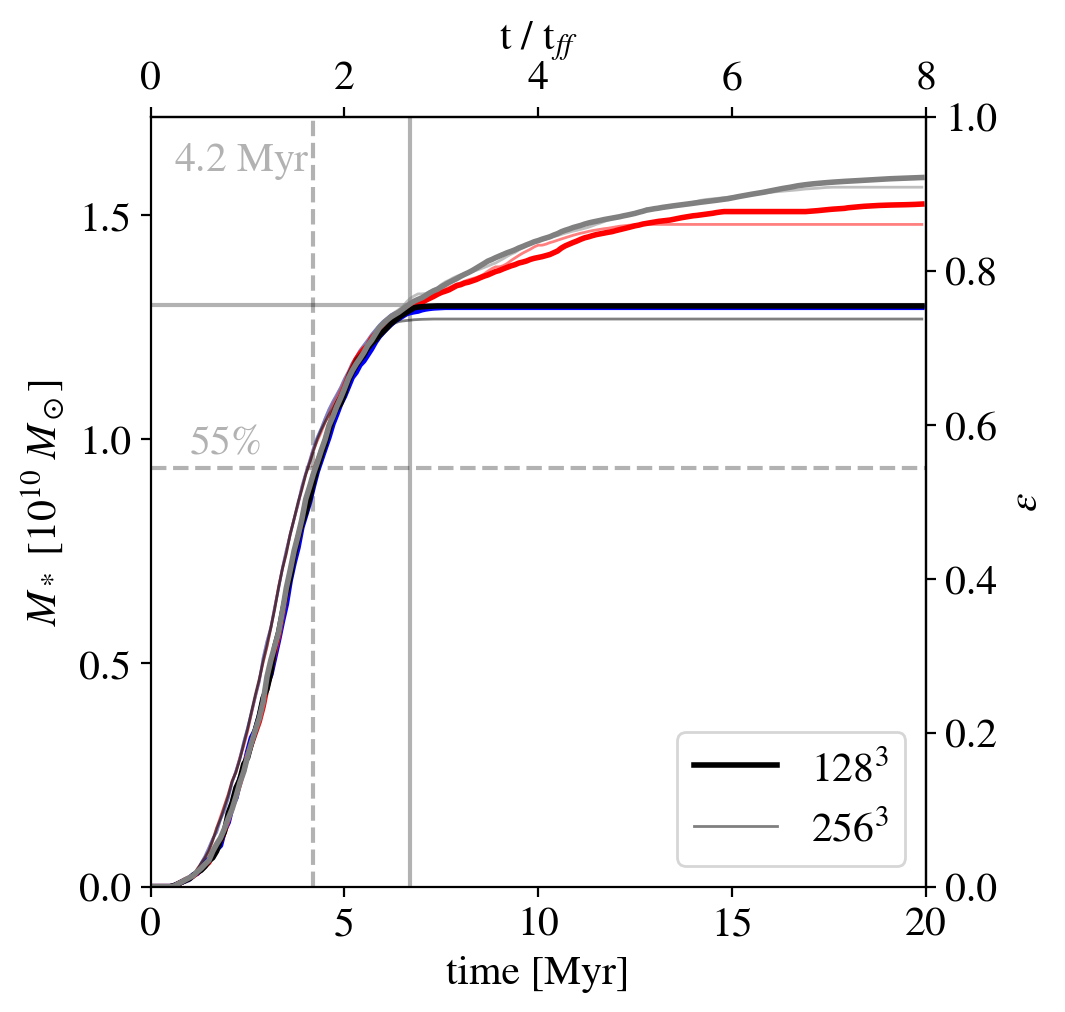
\includegraphics[width=\linewidth]{fig11.png}
    \caption{Stellar mass formed in the simulations as a function of resolution. The line color indicates the feedback physics, and the thickness encodes the resolution of each run. Across all four physics cases, the star formation efficiency is consistent across the resolutions, indicating that the simulations are numerically converged.}
    \label{fig11:Ms_res}
\end{figure}

\section{Summary}
We have presented a suite of three-dimensional radiation hydrodynamic simulations of a gas cloud embedded in a $10^{11}M_\odot$ halo at $z=10$. The clouds are initialized with a mass of $1.7 \times 10^{10} M_\odot \mathrm{pc^{-2}}$, a radius of $700$ pc, and metallicity in selected from $10^{-2}Z_\odot, 10^{-1}Z_\odot$ or $Z_\odot$. We investigate the effects of radiation and supernovae feedback and metallicity on the evolution of the system, and calculate observable signatures. Our main results are as follows.

Due to the high initial gas surface density ($\Sigma_\mathrm{init} > 10^3 M_\odot \ \mathrm{pc^{-2}}$), gravitational collapse dominates the dynamics of the system for the first 6 Myr of the simulation, and star formation occurs essentially unimpeded. Within two freefall times, all the runs have formed $1.3\times 10^{10}\ M_\odot$ ($\epsilon \sim 0.76$) of stellar material (Figure \ref{fig2:sfe}). Star formation occurs unimpeded until the first supernovae detonate at $t = 6.5\ \mathrm{Myr}$, at which point the momentum and energy injected by feedback disperses the ISM (Figure \ref{fig4:postage_fbks}). 

The supernova-driven outflows have mass flux $3\times 10^8 M_\odot\ \mathrm{Myr^{-1}}$, with an average velocity of $1000\ \mathrm{km\ s^{-1}}$ year). At the fiducial metallicity ($10^{-2} Z_\odot$), the winds are energy conserving for the first 10 Myr of detonations, since the gas exits the system faster than it can cool radiatively (Figure \ref{fig6:terminal_mpe_phases}).

The phase structure of the outflowing gas is shaped both by the feedback physics and metallicity of each simulation. Of the total wind mass in the fiducial run, $3\times 10^9 M_\odot)$, $40\%$ is in the WNM, with the remaining $26\%$ in the HIM and $16\%$ in the WIM. While all the cold gas gets destroyed at $0.01 Z_\odot$, $40\%$ of the outflow is in the CNM, due to more efficient cooling and shielding by dust at higher metallicities (Figure \ref{fig7:terminal_mtls_mpe}).

We find that the HIM winds vent at $v > 2 v_\mathrm{esc}$, permanently escaping into the IGM. on the other hand, the warm-phases, which have $v \sim 0.5 v_\mathrm{esc}$, will travel to $1.5-2$ kpc before raining back onto the starburst. 
% within \textcolor{red}{$t=myr$.} 

The temporary clearing of the interstellar gas and dust allows the UV radiation produced by the young starburst to propagate freely. More than $80\%$ of the EUV and $\geq 90\%$ of LW and PE radiation leaves the system, ionizing a bubble of 2.4 Mpc as it propagates into the IGM (Figure \ref{fig8:fesc}).

% \textcolor{red}{our results agree/don't with analytical models proposed to explain the jwst blue monsters. they agree/don't with cosmological zoom-in.}
% \textcolor{red}{overall, this work shows that a $10^{11} M_\odot$ halo at $z = 10$ in a $\lambda$-CDM universe is capable of rapid stellar mass assembly (msun / yr), reaching sfe of (). after $2t\mathrm{ff}$, supernova-driven outflows temporarily clear the gas and dust, rendering visible a UV-bright compact object  of mass = $M_\odot$ and muv.}

\textcolor{cyan}{for the summary section - focus more on the bigger picture - frame as what do the results im reporting mean to a reader who is interested in starbursts in the early universe, less on the technical details of what we simulated. for each section / new topic switch saderg lemn ena endet wedeza endehedn explain mareg. make sure to do a linear read through edit mareg salemer befit to get a sense of where things need to be mroe explicitly stitched together. make sure all the variables / quantities defined in equations i explain mn endehonu. err on the side of explaining - can be inline. put in equation for energy that cs is derived from in section 2.1. reorder the figures to line up with yet how much endamawerachew. numerical experiment of a global burst of star formation - in the abstract and summary how we talk about the set up will be more about mndnew analogize mareg eyemokern yalenew vs in the results we can be more technical - then the connection the jwst systems will be more straightforward. experiment designed (what are the feedback mechanisms and other conditions put in) to mimic observed systems that have (gone through a burst ofo star formation, at high redshift, ...), 'the system', 'the starburst' , general idea: think about who the reader would be / what are the context that they would have} 

\software{astropy \citep{2018AJ....156..123A},  
         matplotlib \citep{2016zndo.....61948D},
         pandas \citep{2022zndo...6053272R}
         scipy \citep{2018zndo...1218715V}
         numpy \citep{harris2020array}
         yt \citep{yt}
         joblib
          }
          
\bibliography{references}{}
\bibliographystyle{aasjournal}

\end{document}

 
